%%%%%%%%%%%%%%%%%%%%%%%%%%%%%%%%%
%%%%%%%%Dokumentdefinition%%%%%%%
%%%%%%%%%%%%%%%%%%%%%%%%%%%%%%%%%
\documentclass[oneside,11pt,a4paper,bibliography=totocnumbered,numbers=noenddot]{scrreprt} 
\usepackage{geometry}
\geometry{a4paper, top=25mm, left=30mm, right=40mm, bottom=25mm, headsep=5mm, footskip=12mm}

%%%%%%%%%%%%%%%%%%%%%%%%%%%%%%%%%%%%%%%%%%%%%%%%%%%
%Inputfile für Packages (hält das Dokument sauber)%
%%%%%%%%%%%%%%%%%%%%%%%%%%%%%%%%%%%%%%%%%%%%%%%%%%%
%%%%%%%%%%%%%%%%%%%%%%%%%%%%%%%
%Kopf- und Fußzeilendefinition%
%%%%%%%%%%%%%%%%%%%%%%%%%%%%%%%
\usepackage[headsepline,footsepline]{scrlayer-scrpage}	%mit Trennlinien
\pagestyle{scrheadings}					%Seitenstil umdefiniert
\clearscrheadfoot					%Definition leermachen
\renewcommand{\chapterpagestyle}{scrheadings}		%Kapitelseitenstil umdefiniert
\renewcommand{\chaptermark}[1]{\markboth{\ #1}{}}	%Definition Kapitel?berschrift=\leftmark
\ohead{\leftmark}				%äußere Kopfzeile
\chead{}						%mittlere Kopfzeile
\ihead{}						%innere Kopfzeile
\ofoot{\thepage}				%äußere Fußzeile
\cfoot{}						%mittlere Fußzeile
\ifoot{}						%innere Fußzeile

%%%%%%%%%%%%%%%%%%%%%%%%%%%%%%%%%%%%%%%
%%%%%%%deutsche Zeichenkodierung%%%%%%%
%%%%%%%%%%%%%%%%%%%%%%%%%%%%%%%%%%%%%%%
\usepackage[utf8]{inputenc}
\usepackage[english,ngerman]{babel} 

%%%%%%%%%%%%%%%%%%%%%%%%%%%%%%%%%%%%%%%%%%%%%%
%%%%%%%%%%%%Verschiedene Schriftarten%%%%%%%%%
%%%%%%%%%%%%%%%%%%%%%%%%%%%%%%%%%%%%%%%%%%%%%%
%\usepackage{crimson}
%\usepackage[adobe-utopia]{mathdesign}
%\usepackage{libertine}
%\usepackage{lmodern}
\usepackage{kpfonts}
%\usepackage{stix}
%\usepackage{libertinust1math}
\usepackage[T1]{fontenc}
%\renewcommand*\familydefault{\sfdefault}

%%%%%%%%%%%%%%%%%%%%%%%%%%%%%%%%%%%%%%%%%%%%%%
%%%%%%%%%%%%%%%Zusatzpackages%%%%%%%%%%%%%%%%%
%%%%%%%%%%%%%%%%%%%%%%%%%%%%%%%%%%%%%%%%%%%%%%
\usepackage{a4wide}
\usepackage{longtable}
\usepackage{csquotes}
\usepackage{longtable}
\usepackage[locale=DE]{siunitx}
\usepackage{eurosym}					%Fancy ? Zeichen
\usepackage{acronym}					%Abk?rzungsverzeichnis
\usepackage{wasysym}					%Symbole und Sonderzeichen
\usepackage{longtable}					%Formelzeichentabelle/lange Tabelle
\usepackage{romannum}					%R?mische Zahlen
\usepackage{wrapfig}					%Bilder nebeneinander/ Text neben Bild
\usepackage{floatflt,epsfig} 				%Bilder im eps-format einf?gen
\usepackage{exceltex}					%Exceldokumente einbinden
\usepackage{multirow}					%Tabellenzellen verbinden
\usepackage{graphicx}					%ich glaube ein Vektorzeichentool
\usepackage[hyphens]{url}				%Websites einbinden
\usepackage{pdfpages} 					%direkt pdf Datein einbinden
\usepackage{amsmath}					%matheumgebung f?r Formeln und Gleichungen
\usepackage{booktabs}					%ich glaube f?r links im PDF
\usepackage{capt-of}					%Captions f?r non-float-Objekte
\usepackage{appendix}					%erm?glicht das erstellen von Anhangsverzeichnissen
\usepackage{listings}
\renewcommand{\lstlistlistingname}{Codeverzeichnis}
\renewcommand{\lstlistingname}{Quellcode}
\usepackage{xcolor}
\usepackage{tikz}					%tikz Paket f?r Grafiken + Definitionen
\usetikzlibrary{arrows,positioning}
\usetikzlibrary{decorations.pathmorphing}
\usetikzlibrary{shapes.geometric}
\usepackage{svg}
\usepackage{caption}

%%%%%%%%%%%%%%%%%%%%%%%%%%%%%%%%%%%%%%%%
%%%%Stil des Literaturverzeichnisses%%%%
%%%%%%%%%%%%%%%%%%%%%%%%%%%%%%%%%%%%%%%%
%\bibliographystyle{abbrvdin}		%sortiert nach Autor 		- nummeriert [1]
%\bibliographystyle{unsrtdin}		%sortiert nach Textmarke	- nummeriert [1]
\bibliographystyle{alphadin}		%sortiert nach Autor		- [AUTOR-JAHR]


%%%%%%%%%%%%%%%%%%%%%%%%%%%%%%%%%%%%%%%%%
%%%%%%%%%%%%%%special Stuff%%%%%%%%%%%%%%
%%%%%%%%%%%%%%%%%%%%%%%%%%%%%%%%%%%%%%%%%
\usepackage[colorlinks,    				%PDF linked Verzeichnis
pdfpagelabels,
pdfstartview = FitH,
bookmarksopen = true,
bookmarksnumbered = true,
linkcolor = black,
plainpages = false,
hypertexnames = false,
citecolor = black,
breaklinks = true,
allcolors = black] {hyperref}  

% custom caption command thingy to cite if needed
% vspace -11 to force effective single spacing between caption and src
\newcommand{\source}[1]{\vspace{-11pt} \caption*{ Quelle: {#1}} }

%\renewcommand{\labelitemi}{-}   %aufzählungszeichen strich statt punkt - beliebig anpassbar
\definecolor{codegreen}{rgb}{0,0.6,0}
\definecolor{codegray}{rgb}{0.5,0.5,0.5}
\definecolor{codepurple}{rgb}{0.58,0,0.82}
\definecolor{backcolour}{rgb}{0.95,0.95,0.92}

\definecolor{whitecolour}{rgb}{1.00,1.00,1.00}

\lstdefinestyle{STYLE_COMMAND_LINE_ARGUMENT_SINGLE_LINE}{
    backgroundcolor=\color{whitecolour},
    keywordstyle=\color{backcolour},
    basicstyle=\ttfamily\small,
    breakatwhitespace=false,         
    breaklines=true,                 
    captionpos=b,                    
    keepspaces=true,                 
    numbers=none,                    
    numbersep=0pt,                  
    showspaces=false,                
    showstringspaces=false,
    showtabs=false,                  
    tabsize=2,
    frame=tb,
    xleftmargin=0.5cm,
    xrightmargin=0.5cm,
}

\lstdefinestyle{STYLE_CODE_JS}{
    backgroundcolor=\color{backcolour},   
    commentstyle=\color{codegreen},
    keywordstyle=\color{magenta},
    numberstyle=\tiny\color{codegray},
    stringstyle=\color{codepurple},
    basicstyle=\ttfamily\footnotesize,
    breakatwhitespace=false,         
    breaklines=true,                 
    captionpos=b,                    
    keepspaces=true,                 
    numbers=left,                    
    numbersep=5pt,                  
    showspaces=false,                
    showstringspaces=false,
    showtabs=false,                  
    tabsize=2
}
\lstset{style=STYLE_CODE_JS}

% \newcommand{\ra}[1]{\renewcommand{\arraystretch}{#1}}

% nicht alle wörter breaken...
\tolerance=1
\emergencystretch=\maxdimen
\hyphenpenalty=10000
\hbadness=10000 			


%\sloppy 					%"schlampiger" Blocksatz
\parindent0cm 					%Absatzeinzug

\usepackage{setspace} 				%Zeilenabstand
%\setstretch{1.2}
\onehalfspacing
%\singlespacing
%\doublespacing

%%%%%%%%%%%%%%%%%%%%%%%%%%%%%%%%%%%%%%%
%hier startet das eigentliche Dokument%
%%%%%%%%%%%%%%%%%%%%%%%%%%%%%%%%%%%%%%%
\begin{document} 					
\begin{titlepage}					%gesondert formatierte Titelseite
\thispagestyle{empty}
\begin{center}



\includegraphics[height=3cm]{bilder/frauaslogo.png}
\begin{figure}[h!]
\centering
\end{figure}\\[1,5cm]

\begin{Large}
\textsf{\textbf{Frankfurt University of Applied Sciences}}\\
\textsf{\textbf{Fachbereich 2: Informatik}}\\[2cm]
\end{Large}


\begin{LARGE}
\textsf{\textbf{Bachelorthesis}}\\
\end{LARGE}
\textsf{zur Erlangung des akademischen Grades Bachelor of Science}\\[1cm]

\begin{Large}
\textsf{\textbf{Einsatz von WebRTC für Browserbasierte Brettspiele im Vergleich zu Client-Server Infrastruktur}}\\[3,5cm]
\end{Large}
\end{center}

\begin{large}
\textsf{Autor: Robin Buhlmann}\\[0,1cm]
\textsf{Matrikelnummer.: 1218574}\\[0,1cm]
\textsf{Referent: Prof. Dr. Eicke Godehardt}\\[0,1cm]
\textsf{Korreferent: Prof. Dr. Christian Baun}\\[0,7cm]
%\textsf{In Kooperation mit: }\\[1,0cm]
\textsf{Version vom: \today}
\end{large}
 			%extrenes .tex Dokument als Titelblatt 
\end{titlepage}
\thispagestyle{empty}
\cleardoublepage
\pagenumbering{Roman}				%Seitennummerierung auf römisch geändert

%\includepdf[pages=-]{} 					%Aufgabenstellung als PDF einbindenfile
%\chapter*{Aufgabenstellung}
%\addcontentsline{toc}{chapter}{Aufgabenstellung}
%\pagebreak

%%%%%%%%%%%%%%%%%%%%%%%%%%%%%%%%%%%%%%%%%%%%%%%%%%%%%%%%%%%%%%%%%%%%%%
\newpage
\chapter*{Eidesstattliche Erklärung}
\chaptermark{Eidesstattliche Erklärung}
\addcontentsline{toc}{chapter}{Eidesstattliche Erklärung}

Hiermit erkläre ich, Robin Buhlmann, dass ich die vorliegende Bachelorarbeit selbstständig und ohne unerlaubte Hilfe angefertigt, andere als die angegebenen Quellen und Hilfsmittel nicht benutzt und die den benutzten Quellen wörtlich oder inhaltlich entnommenen Stellen als solche kenntlich gemacht habe.

Die Arbeit wurde bisher in gleicher oder ähnlicher Form keiner anderen Prüfungsbehörde vorgelegt und auch nicht veröffentlicht.


\vspace{1cm}

Friedrichsdorf, den

\vspace{1cm}

------------------------------------\hspace{6cm}------------------------------------\\
Datum \hspace{9,4cm} Unterschrift

\newpage

\chapter*{Abstract}
\chaptermark{Abstract}
\addcontentsline{toc}{chapter}{Abstract}
%\section*{Abstract}
%warum ist das thema relevant?
%arbeitsumfeld: typo3 super kurz info, bietet php extensions
%ziel der arbeit? in dieser ba soll prototypisch ein ... bewerbungsprozess umgesetzt und evaluiert werden
%1-2 sätze konzepte, "dabei kommen konzepte des CMS, php, mvc blabla
%am ende dieser arbeit steht die evaluation, die zeigt,dass der umgesetzte prototyp alle kriterien erfüllt ist











%Vorwort, Editorial, Erklärungen, Vermerke%%
%%%%%%%%%%%%%%%%%%%%%%%%%%%%%%%%%%%%%%%%%%%%%%%%%%%%%%%%%%%%%%%%%%%%%%


\newpage
\begin{singlespace}

%%%%%%%%%%%%%%%%%%%%%%%%%%%%%%%%%%%%%%%%%%%
%%%%%%%%%%%%%%%Verzeichnisse%%%%%%%%%%%%%%%
%%%%%%%%%%%%%%%%%%%%%%%%%%%%%%%%%%%%%%%%%%%
\setcounter{secnumdepth}{2} 	%countertiefe für Verzeichnisse
\setcounter{tocdepth}{2}		%Auflistungstiefe für Verzeichnisse
\chaptermark{Inhaltsverzeichnis}
\tableofcontents 						%Befehl für Inhaltsverzeichnis
\newpage
\listoffigures 							%Befehl für Abbildungsverzeichnis
\addcontentsline{toc}{chapter}{Abbildungsverzeichnis} 		
\chaptermark{Abbildungsverzeichnis}
\newpage
\listoftables							%Befehl für Tabellenverzeichnis
\addcontentsline{toc}{chapter}{Tabellenverzeichnis}
\chaptermark{Tabellenverzeichnis}
\newpage
\lstlistoflistings
\addcontentsline{toc}{chapter}{Codeverzeichnis}
\chaptermark{Codeverzeichnis}
\newpage

\chapter*{Abkürzungsverzeichnis}	
\addcontentsline{toc}{chapter}{Abkürzungsverzeichnis}
\chaptermark{Abkürzungsverzeichnis}
\begin{acronym}[TDMA]\itemsep0pt

\acro{W3C}{World Wide Web Consortium}
\acro{RTC}{Real-Time Communication}
\acro{WebRTC}{Web Real-Time Communication}
\acro{P2P}{Peer-To-Peer}
\acro{HTTP}{Hypertext Transfer Protocol}
\acro{NPM}{Node Package Manager}
\acro{IETF}{Internet Engineering Task Force}
\acro{RTP}{Real-Time Transport Protocol}
\acro{SRTP}{Secure Real-Time Transport Protocol}
\acro{JSEP}{JavaScript Session Establishment Protocol}
\acro{ICE}{Interactive Connectivity Establishment}
\acro{NAT}{Network Address Translation}
\acro{STUN}{Session Traversal Utilities for NAT}
\acro{TURN}{Traversal Using Relays around NAT}
\acro{SCTP}{Stream Control Transport Protocol}
\acro{TLS}{Transport Layer Security}
\acro{DTLS}{Datagram Transport Layer Security}
\acro{API}{Application Programming Interface}
\acro{TCP}{Transmission Control Protocol}
\acro{UDP}{User Datagram Protocol}
\acro{OSI}{Open Systems Interconnection}
\acro{IP}{Internet Protocol}
\acro{SDK}{Source Development Kit}
\acro{SIP}{Session Initialization Protocol}
\acro{SDP}{Session Description Protocol}
\acro{URI}{Unique Resource Identifier}
\acro{URL}{Unique Resource Locator}
\acro{HTML}{Hypertext Markup Language}
\acro{VM}{Virtuelle Maschine}
\acro{RTMFP}{Real-Time Media Flow Protocol}
\acro{RC4}{Rivest Cipher 4}
\acro{HMAC}{Hash-Based Message Authentication Code}
\acro{SHA-1}{Secure Hash Algorithm 1}
\acro{JSON}{JavaScript Object Notation}
\acro{DOM}{Document Object Model}

\end{acronym}
\end{singlespace}

\cleardoublepage
\pagenumbering{arabic}			%ab hier arabische Seitenzahlen

%Vorlagenkapitel
\chapter{Einleitung}
\section{Motivation}
\section{Zielsetzung}
\section{Aufbau der Arbeit}

\chapter{Grundlagen}
% TODO: vllt dieses kapitel auf dateien teilen, is ziemlich lang
In diesem Kapitel werden die zum Verständnis der Implementierung benötigten theoretischen, sowie technischen Grundlagen beschrieben. Dabei werden primär die Funktionalität von \acs{WebRTC} an sich, als auch die damit verbundenen Signal-Mechanismen und Infrastrukturen behandelt.

\section{Echtzeitanwendungen}
Unter den Begriff Echtzeitanwendung fällt prinzipiell jede Anwendung, deren von Nutzern ausgelöste Ereignisse nur gewisse, in der Regel für den Nutzer nicht wahrnehmbare Verzögerungen aufweisen dürfen. Ein Beispiel für Echtzeitanwendungen sind Audio- und Videokommunikationsprogramme. Die Audio- und Videodaten müssen schnellstmöglich zwischen den Teilnehmern eines Anrufs ausgetauscht werden, um den Eindruck zu vermitteln, dass die Gesprächsteilnehmer direkt miteinander sprechen. Spricht zum Beispiel eine Person, so muss der Ton zur nahezu gleichen Zeit bei allen anderen Personen, welche dem Anruf teilhaben, ankommen.

\section{Netzwerkarchitekturen}

\subsection{Client-Server-Modelle}
Eine Client-Server Netzwerktopographie setzt sich aus primär zwei Arten an Knoten zusammen: Clients und Servern. Ein Server hat die Aufgabe, den Clients Daten und Services zur Verfügung zu stellen \cite{silveira2015}. In der Regel kann ein Server dabei eine Vielzahl an Clients versorgen.\par

\subsubsection{Web-Architektur}
Die Architektur von Webanwendungen basiert in der Regel auf auf einem Client-Server-Modell, wobei der Browser des Clients \acf{HTTP}-Anfragen an den Server sendet, um Inhalte vom Server abzurufen. Diese Inhalte lassen sich anhand eines \acf{URI}, beziehungsweise einer \acf{URL} abrufen. Die Webanwendung kann zudem durch JavaScipt-Code mit eingebetteten \acf{API}s der Browser interagieren \cite{lorento2014}.\par

\subsubsection{Authoritative-Server}
Bei der Entwicklung von Mehrspieler-Spielen wird oftmals das sogenannte \glqq{}Authoritative-Server\grqq{}-Modell verwendet. Dabei ist ein Zentraler Server für die gesamte Verwaltung des Spielstandes zuständig. Die Spieler -- die Clients -- halten lediglich den minimal benötigten Status, um das Spiel darzustellen. Jede Aktion des Spielers, welche den Spielstand beeinflusst -- zum Beispiel das Bewegen einer Spielfigur oder das Ziehen einer Karte -- muss über den Server geregelt und autorisiert werden \cite{authservermodel} (vgl. Abbildung~\ref{figure:authserver}).\par

\begin{figure}[h]
\centering
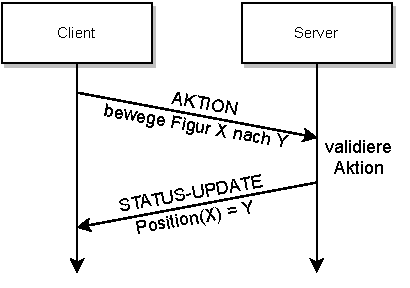
\includegraphics[width=0.65\textwidth]{bilder/PDF_SVG/AUTH_SERVER.pdf}
\caption{Beispielhafte Interaktion in einem Authoritative-Server-Modell.}
\label{figure:authserver}
\end{figure}

Dieser Ansatz eignet sich besonders für Spiele, in welchen Spieler nicht durch unerlaubte Modifikation der Spieldateien Vorteile verschaffen dürfen. Da alle Aktionen über den Server geregelt werden, ist es einfach unerlaubte Änderungen am Spielstand zu verbieten \cite{authservermodel}.\par

\subsection{Peer-To-Peer Netzwerke}

\section{Network Address Translation}

\section{Web Real-Time-Communication}
Bei \ac{WebRTC} handelt es sich um einen Quelloffenen Standard zur Echtzeitkommunikation zwischen Browsern. Im Gegensatz zu weiteren Echtzeitstandards, wie zum Beispiel WebSockets, setzt \acs{WebRTC} nicht auf ein Client-Server Modell. Stattdessen ermöglicht der Standard es Browsern, welche den \acs{WebRTC} Standard unterstützen, sich ohne zusätzliche Software oder Plugins direkt miteinander zu verbinden. Der Datenaustausch findet somit direkt zwischen den Browsern -- den sogenannten Peers -- statt, ohne dass die Daten zusätzlich über einen Server weitergeleitet werden müssen. Dies führt in der Regel zu geringeren Latenzen, sowie Kostenersparnissen durch weniger Serverlast. WebRTC ist primär auf Audio- und Videokommunikation ausgelegt, ermöglicht aber auch das Senden von arbitraren Daten.\par

Der Standard wurde zuerst von Global IP Solutions (GIPS) entwickelt. In 2011 erwarb Google GIPS, machte die \acs{WebRTC}-Komponenten Open-Source, und ermöglichte die Integration der Technologie in Web-Browsern durch die Entwicklung einer JavaScript-\acs{API}. Seitdem arbeitet das \acs{W3C} an der Standardisierung der Technologie.

Der Standard wird nun von einer Arbeitsgruppe des \acs{W3C}, der \acs{WebRTC} Working Group (dt. WebRTC Arbeitsgruppe) entwickelt und erhalten. Insgesamt 18 Organisationen sind in der WebRTC Arbeitsgruppe vertreten, unter anderem Microsoft, Google, Mozilla, Cisco und Apple \cite{webRTCWorkingGroup}.\par

Am 26. Januar 2021 veröffentlichte das \acs{W3C} die \acs{WebRTC}-Recommendation -- \acs{WebRTC} ist damit ein offizieller, vom \acs{W3C} befürworteter Web-Standard, welcher für eine weitverbreitete Verwendung bereit ist. 

\subsection{Aufbau von WebRTC}
WebRTC ist kein proprietärer, einzelner und zusammenhängender Standard, sondern eine Ansammlung bereits existierender Protokolle, Technologien und Standards, welche unter anderem den Aufbau von Verbindungen, Audio- und Videoübertragung, sowie Datenübertragung regeln.\par

\begin{figure}[h]
\centering
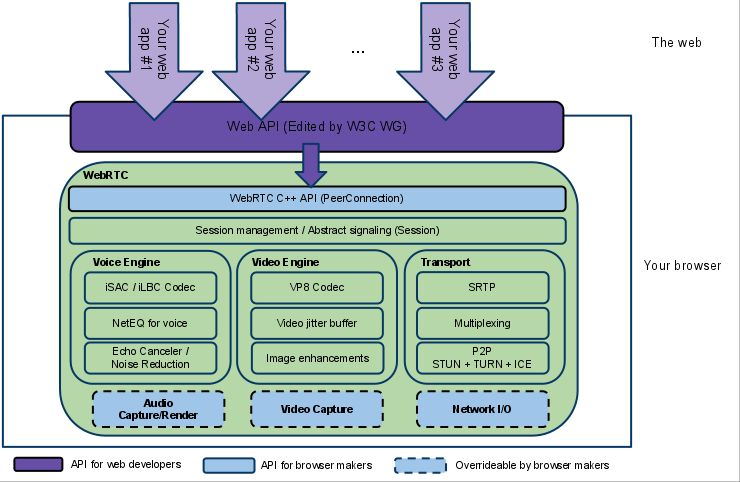
\includegraphics[width=0.95\textwidth]{bilder/webrtc-diagram.png}
\caption{Diagramm der WebRTC-Architektur.}
\source{\url{https://webrtc.github.io/webrtc-org/architecture/}}
\label{fig:webrtcArchitecture}
\end{figure}

Wie dem Architekturdiagramm in Abbildung ~\ref{fig:webrtcArchitecture} zu entnehmen, gliedert sich WebRTC primär in eine Web-\acs{API} und das \acs{WebRTC}-Framework. Hinzu kommen Signalisierungsmechanismen, welche zum Aufbau einer Verbindung benötigt werden. Diese sind nicht durch den WebRTC-Standard vorgeschrieben. Es ist dem Entwickler überlassen, wie die Signalisierung letztendlich implementiert wird -- es muss lediglich möglich sein, Daten zur Sitzunsinitialisierung zwischen jeweils zwei Peers auszutauschen.\par

\subsubsection*{Web-API}
Die Web-\acs{API} dient dabei zur Entwicklung von Browserbasierten Webanwendungen, und setzt sich aus einer Reihe an JavaScript Schnittstellen zusammen. Diese Schnittstellen können auf das unterliegende Framework zugreifen, und ermöglichen zum Beispiel das Erstellen von Verbindungen, Datenkanälen und Video-Streams. Primär werden dabei die folgenden Schnittstellen verwendet:

\begin{itemize}
  \item Die \textbf{RTCPeerConnection}-Schnittstelle repräsentiert eine WebRTC-Verbindung zwischen dem lokalen Browser (Local-Peer), und einem externen Browser (Remote-Peer) \cite{rtcpeerconnection}. Die Signalisierungsmechanismen folgen dabei dem \ac{JSEP}, die Verbindung selbst wird via dem \ac{ICE} Framework hergestellt \cite{loreto2014}.
  
  \item Ein \textbf{RTCDataChannel} ist ein, von der RTCPeerConnection erstellter, bidirektionaler Datenkanal, welcher den Austausch von arbitraren Nachrichten zwischen Browsern ermöglicht. Eine RTCPeerConnection kann mehrere Datenkanäle besitzen. Zum Datenaustausch wird das \ac{SCTP} verwendet \cite{loreto2014, rtcpeerconnection}.
  
  \item Die \textbf{MediaStream}-\acs{API} dient dazu, Audio- und Videosignale eines Gerätes abzurufen. Dabei wird ein Datenstrom erzeugt, welcher in Echtzeit an externe Browser gesendet werden kann. Dazu wird das \ac{RTP}, beziehungsweise das \ac{SRTP} verwendet \cite{loreto2014}. Da Audio- und Videoübertragung für diese Arbeit nicht relevant sind, wird auf diese Protokolle nicht weiter eingegangen.
\end{itemize}

\subsubsection*{WebRTC Framework}
Das \acs{WebRTC}-Framework gliedert sich primär in Audio- Video- und Übertragungssysteme. Die Audio- und Videosysteme befassen sich dabei unter anderem mit der Abfrage von Audiodaten des Gerätemikrofons, sowie Videodaten über eine Kamera, welche an das Gerät angeschlossen ist. Zudem sind diese Systeme für die en- und decodierung von Audio- und Videodaten auf Basis verschiedener \glqq{}Codecs\grqq{} zuständig. Auf diese wird hier nicht weiter eingegangen.\par

Die Transportsysteme umfassen Protokolle und Systeme, um Sitzungen zwischen Peers aufzubauen, und Daten zwischen den Peers zu versenden. Die Sitzungskomponenten basieren dabei auf \glqq{}libjingle\grqq{}, einem Quelloffenen C++ \ac{SDK}, welches das Erstellen von Peer-To-Peer Sitzungen ermöglicht. Hinzu kommen Protkolle wie \acs{STUN}, \acs{TURN} und \acs{ICE}, welche in den Folgenden Unterpunkten näher erläutert werden.

%\subsection{Protokolle und Frameworks}
%Die mit der Implementierung zusammenhängenden Protokolle werden im %Fogenden näher erläutert -- sowohl deren Funktionalität, als auch deren %Zusammenspiel untereinander.\par

\subsection{JSEP: JavaScript Session Establishment Protocol}
Die Signalisierungsebene einer \acs{WebRTC}-Anwendung ist nicht vom \acs{WebRTC}-Standard definiert, damit verschiedene Applikationen mitunter verschiedene Signalisierungsprotkolle, wie zu Beispiel das \acf{SIP}, oder ein proprietäres Protokoll nutzen können.\par

Das \acf{JSEP} erlaubt es einem Entwickler, die volle Kontrolle über die unterliegende Zustandsmaschine des Signalisierungsprozesses zu haben, welche die Initialisierung einer Sitzung kontrolliert. Damit werden die Signalisierungs- und Datenübertragungsebene effektiv voneinander getrennt. Eine Sitzung wird immer zwischen zwei Endpunkten etabliert, einem initiierendem Endpunkt, und einem empfangenden Endpunkt. In den folgenden Paragraphen werden die Synonyme \glqq{}Alice\grqq{} und \glqq{}Bob\grqq{} für diese Endpunkte verwendet.\par

Beide Endpunkte besitzen dabei jeweils eine lokale, und eine externe Konfiguration (eng. \glqq{}localDescription\grqq{} und \glqq{}remoteDescription\grqq{}). Diese definieren die Sitzungsparameter, zum Beispiel welche Daten auf der Senderseite versendet werden sollen, beziehungsweise welche Daten auf der Empfängerseite zu erwarten sind, oder Informationen über verwendete Audio- und Videocodecs. Diese Informationen werden über das \acf{SDP} definiert.\par

Die \acs{JSEP}-\acs{API} stellt dazu eine Reihe an asynchronen Funktionen zur Verfügung, welche das Erstellen und Setzen der Konfigurationen ermöglichen. Diese Funktionen sind in der \acs{WebRTC}-\acs{API} Teil der RTCPeerConnection.\par

\begin{figure}[h]
\centering
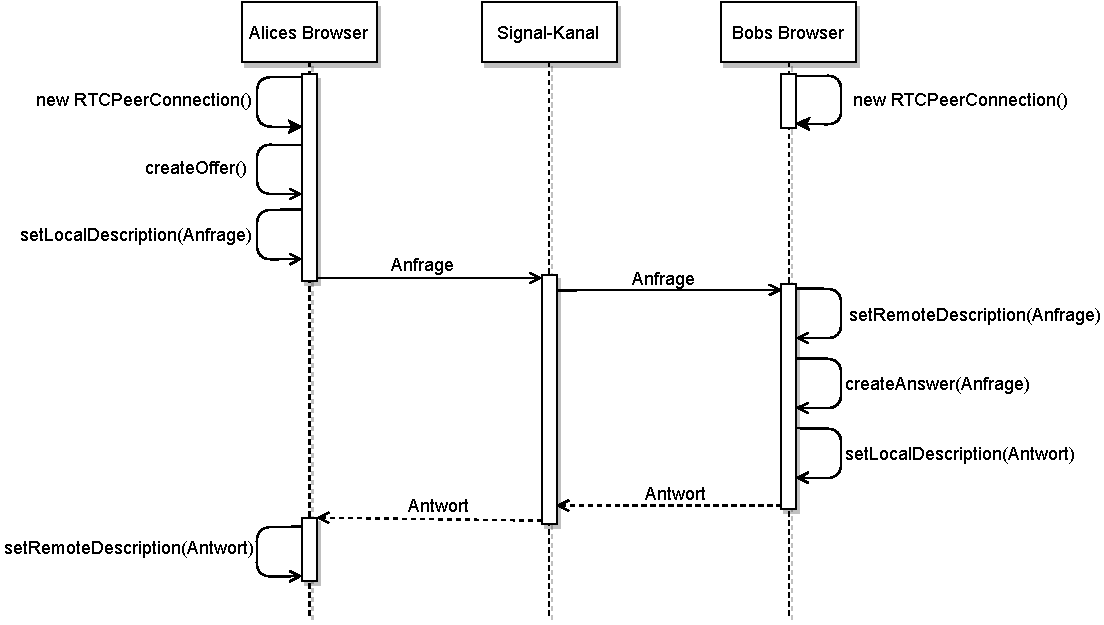
\includegraphics[width=0.95\textwidth]{bilder/PDF_SVG/JSEP.pdf}
\caption{\acs{JSEP}-Verbindungsaufbau.}
\label{fig:jsep}
\end{figure}

Um eine Verbindung aufzubauen, ruft Alice erst \textit{createOffer()} auf. Daraufhin wird ein SDP-Packet (\textit{anfrage}) generiert, welches die lokalen Sitzungsparameter enthält. Alice setzt nun ihre lokale Konfiguration via \textit{setLocalDescription(anfrage)}. Das \acs{SDP}-Packet wird über einen nicht vorgegebenen Signalkanal zu Bob gesendet. Dieser setzt daraufhin die externe Konfiguration seiner Verbindung via \textit{setRemoteDescription(anfrage)}, und ruft daraufhin die Funktion \textit{createAnswer(anfrage)} auf, welche eine Antwort (\textit{antwort}) generiert. Bob setzt seine lokale Konfiguration via \textit{setLocalDescription(antwort)}, und sendet die Antwort zurück zu Alice. Alice setzt ihre externe Konfiguration via \textit{setRemoteDescription(antwort)}. Damit ist der anfängliche Austausch von Sitzungsparametern abgeschlossen \cite{altanai2014}. \acs{JSEP} regelt dabei nur den Austausch von Konfigurationen zwischen zwei Peers, Informationen über die Verbindung werden über das \acs{ICE}-Framework ausgetauscht. Der vereinfachte Ablauf des Verbindungsaufbaus ist Abbildung ~\ref{fig:jsep} zu entnehmen.

\subsection{ICE: Interactive Connectivity Establishment}
Das \acf{ICE}-Framework erlaubt es Browsern (Peers), Verbindungen untereinander aufzubauen. Es wird benötigt, da dies aufgrund der Tatsache, dass sich Peers in der Regel in einem lokalen Subnetz hinter einem \acs{NAT} (Network Address Translation) befinden, nicht ohne weiteres möglich ist. Das \acs{ICE}-Framework bietet in Kombination mit den Protokollen \acs{STUN} und \acs{TURN} Möglichkeiten, direkte Verbindungen zweier Peers durch \acs{NAT} herzustellen, beziehungsweise Datenverkehr über ein Relais umzuleiten.\par

Eine \acs{WebRTC} Verbindung (RTCPeerConnection) besitzt dabei immer einen sogenannten \acs{ICE}-Agenten, sowohl auf der lokalen, als auch auf der externen Seite. Dabei agiert einer der Agenten einer Verbindung als der kontrollierende, der Andere als der kontrollierte Agent. Der kontrollierende Agent hat dabei die Aufgabe, das \acs{ICE}-Kandidatenpaar, welches für die Verbindung genutzt werden soll, auszuwählen. Ein \acs{ICE}-Kandidat beinhaltet Informationen, im \acs{SDP}-Format, über Transportadressen -- Adress-Port-Tupel --, über welche ein Peer erreicht werden kann. Ein \acs{ICE}-Kandidatenpaar ist ein Paar von zwei \acs{ICE}-Kandidaten, welche zum gegenseitigen Verbindungsaufbau zweier Peers verwendet werden können.

\begin{figure}[h]
\centering
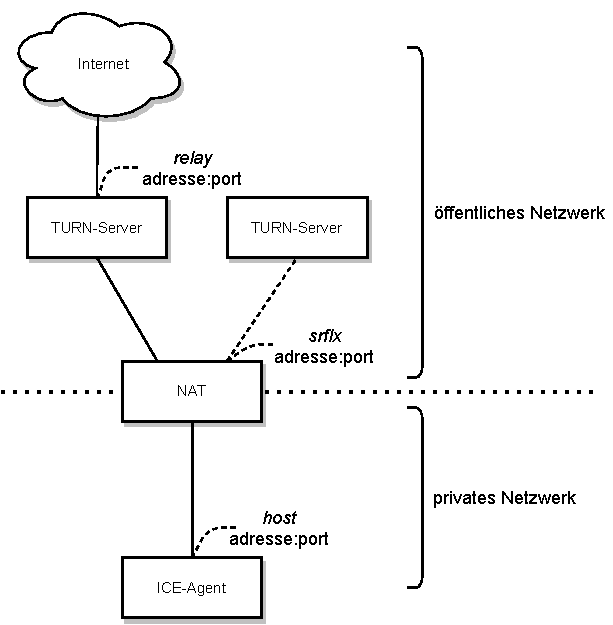
\includegraphics[width=0.80\textwidth]{bilder/PDF_SVG/CANDIDATES_OLD.pdf}
\caption{Diagramm der verschiedenen \acs{ICE}-Kandidaten.}
\source{Angepasst nach \url{https://tools.ietf.org/html/rfc5245}}
\label{fig:icecandidates}
\end{figure}

Ein Gerät hinter einem \acs{NAT} besitzt keine eigene, öffentliche \acs{IP}-Adresse. Ein Peer muss jedoch seine eigene, öffentliche \acs{IP}-Adresse kennen, um dem Verbindungspartner mitteilen zu können, an welche Adresse dieser die Daten schicken soll. In der Regel handelt es sich bei  \acs{ICE}-Kandidaten um \acs{UDP}-Transportadressen. Es existieren zwar auch \acs{TCP}-Kandidaten, diese werden allerdings nicht von allen Browsern unterstützt und in der Regel nicht verwendet. Wie aus Abbildung ~\ref{fig:icecandidates} zu entnehmen, werden dabei primär drei Arten an \acs{UDP}-\acs{ICE}-Kandidaten verwendet:

\begin{itemize}
	\item Ein \textbf{Host}-Kandidat (\textit{typ host}) ist der tatsächliche Adress-Port-Tupel eines Peers. Host-Kandidaten können nur dann verwendet werden, wenn der Peer eine öffentliche \acs{IP}-Adresse besitzt, oder sich sowohl der lokale, als auch externe Peer im gleichen Subnetz, oder auf dem gleichen Gerät befinden.
	\item Ein \textbf{Server-Reflexiver}-Kandidat (\textit{typ srflx}) repräsentiert die öffentliche \acs{IP}-Adresse eines Peers, also die öffentliche \acs{IP}-Adresse des \acs{NAT}s, hinter welchem sich der Peer befindet. Befindet sich der Peer nicht hinter einem \acs{NAT}, so ist die Adresse gleich der Host-Adresse, und der Kandidat wird verworfen.
	\item Ein \textbf{Relais}-Kandidat (\textit{typ relay}) ist ein Adress-Port-Tupel, welcher dem Peer von einem \acs{TURN}-Server zugeordnet wurde. Diese Adresse ist dabei die Adresse, welche der \acs{TURN}-Server nutzt, um eingehende Daten an den Peer, und ausgehende Daten von dem Peer weiterzuleiten.
\end{itemize}

\subsubsection{Trickle-ICE}
Die \acs{STUN} und \acs{TURN} Server lassen sich beim Erstellen der RTCPeerConnection konfigurieren. \acs{WebRTC} prüft die Verbindung zu allen möglichen \acs{ICE}-Kandidaten eines Peers asynchron in Parallel, sobald die lokale Beschreibung einer Verbindung gesetzt ist. Dieser Prozess -- der sogenannte \glqq{}\acs{ICE}-Sammelprozess\grqq{} -- setzt eine Kommunikation mit \acs{STUN}- und \acs{TURN}-Servern vorraus und kann daher, je nach Latenz und Antwortzeit der Server, einige Zeit beanspruchen.\par

Aus diesem Grund ermöglicht es \acs{WebRTC}, \acs{ICE}-Kandidaten zu \glqq{}tricklen\grqq{}, also jeweils einzelne Kandidaten bei Erhalt einer Serverantwort an den externen Peer zu schicken. Dies optimiert den Vorgang des Austauschs von \acs{ICE}-Kandidaten, da der \acs{JSEP}-Anfrage-Antwort-Prozess nun parallel zum \acs{ICE}-Sammelprozess stattfinden kann. Unterstützt ein älterer Browser kein \glqq{}Trickle-\acs{ICE}\grqq{}, so müssen vor dem Abschicken der \acs{JSEP}-Anfrage oder Antwort alle \acs{ICE}-Kandidaten gesammelt, und den \acs{SDP}-Daten der jeweiligen Nachricht beigefügt sein.\par

\vspace{1pc}
\lstset{style=STYLE_ICE_CANDIDATE_0}
\begin{lstlisting}[caption={SDP-Datenstring eines Relais-ICE-Kandidaten},captionpos=b,label={lst:candidate}]
candidate:1411127089 1 udp 33562367 <@\textcolor{blue}{20.56.95.156}@> <@\textcolor{blue}{12926}@> <@\textcolor{red}{typ}@> <@\textcolor{red}{relay}@> raddr 0.0.0.0 rport 0 generation 0 ufrag uVtu network-cost 999
\end{lstlisting}

Jede RTCPeerConnection besitzt daher die Rückruffunktion \glqq{}$onicecandidate$\grqq{}, welche bei Erhalt eines neuen \acs{ICE}-Kandidaten aufgerufen wird. Die Parameter dieser Rückruffunktion enthalten die \acs{SDP}-Daten, welche den Kandidaten beschreiben. Die Struktur dieser Daten ist Beispielhaft Abbildung~\ref{lst:candidate} zu entnehmen. Dabei handelt es sich um einen \acs{UDP}-Relais-Kandidaten, zu erkennen am \glqq{}typ relay\grqq{}, hervorgehoben in Rot. Die Adresse und der Port sind in Blau hervorgehoben. Der Kandidat wird automatisch zur lokalen Beschreibung des Peers, welcher den Kandidaten fand, hinzugefügt. Nachdem die Daten daraufhin an den externen Peer gesendet wurden, muss der Kandidat auf der Empfängerseite über die $addIceCandidate$-Funktion der externen Konfiguration der RTCPeerConnection hinzugefügt werden.

\subsubsection{STUN: Session Traversal Utilities for NAT}
Das \acf{STUN}-Protokoll wird verwendet, um die öffentliche \acs{IP}-Adresse eines Peers zu ermitteln. Auf Anfrage an einen STUN-Server erhält ein Peer seine Server-Reflexive Transportadresse zurück, welche von externen Peers verwendet werden kann, um Daten an den lokalen Peer zu schicken. Durch die Anfrage an den \acs{STUN}-Server wird dabei die benötigte Port- und Adresszuordnung in die \acs{NAT}-Übersetzungstabelle des Routers geschrieben. Eine Server-Reflexive Adresse kann auch von einem TURN-Server abgefragt werden, vorrausgesetzt dieser unterstützt zusätzlich das \acs{STUN}-Protokoll.\par

\subsubsection{TURN: Traversal Using Relays around NAT}
Im Gegensatz zu Client-Server-Verbindungen, welche nur vom Client eröffnet werden können, kann eine Peer-To-Peer Verbindung zudem sowohl vom lokalen Peer, als auch von einem Peer außerhalb des lokalen Subnetzes eröffnet werden. Hier besteht das Problem, dass nicht jede Art von \acs{NAT} das Eröffnen einer Verbindung von Außerhalb erlaubt \cite{natproblemsRFC}.\par

An diesem Punkt setzt das \acf{TURN}-Protokoll an. Ein \acs{TURN}-Server ermöglicht es, Daten, welche von einem externen Peer an den \acs{TURN}-Server geschickt wurden, an einen Peer weiterzuleiten. Zudem kann der Peer Daten an den Turn-Server schicken, welche wiederrum an externe Peers weitergeleitet werden. Ein TURN-Server agiert somit als ein zwischen den Peers liegender Relais-Server, für Fälle, in denen eine direkte Verbindung zwischen Peers aufgrund von \acs{NAT}-Einschränkungen nicht möglich ist.

\subsection{SCTP: Stream Control Transmission Protocol}
Zur Übertragung von Daten via RTCDataChannels nutzt \acs{WebRTC} das \acf{SCTP}. Der \acs{SCTP} Standard wurde erstmals im Jahre 2000 von der \acs{IETF} veröffentlicht, und seitdem weiterentwickelt und erweitert. \acs{SCTP} ist ein zuverlässiges, Nachrichtenorientiertes Transportprotokoll, welches im \acf{OSI}-Referenzmodell, ähnlich wie \acs{UDP} oder \acs{TCP}, auf der Transportschicht liegt. Das Protokoll arbeitet dabei basierend auf verbindungslosen Netzwerkprotokollen wie zum Beispiel dem \acf{IP} \cite{sctpRFC}.\par

Im Gegensatz zu \acs{TCP} und \acs{UDP} lassen sich bei \acs{SCTP}, je nach gewünschter Verbindungsart, die folgenden Aspekte unabhängig voneinander frei konfigurieren:
\begin{itemize}
	\item\textbf{Reihenfolge}: \acs{SCTP} ermöglicht es, sowohl geordnete, als auch ungeordnete Datenströme aufzubauen. Falls ein Datenstrom geordnet ist, so müssen die Datenpakete in der Reihenfolge beim Empfänger ankommen, wie sie vom Sender losgeschickt wurden. In ungeordneten Datenströmen ist die Reihenfolge der Pakete, wie sie beim Empfänger ankommen, nicht relevant \cite{sctpRFC}.
	\item\textbf{Zuverlässigkeit}: Die Zuverlässigkeit der Paketlieferungen ist auf zwei Arten konfigurierbar. Es ist möglich, eine maximale Anzahl an Versuchen festzulegen, mit welcher versucht wird, ein Datenpaket zu versenden. Zudem kann eine maximale Lebenszeit für Pakete angegeben werden. Ist diese Lebenszeit, das sogenannte 'Retransmission Timeout' für eine Paketsendung abgelaufen, so wird kein weiterer Versuch unternommen, das Paket abzuschicken \cite{sctpRFC}.
\end{itemize}

\vspace{11pt}

Im Gegensatz zu \acs{TCP} und \acs{UDP} ermöglicht \acs{SCTP} Multiplexing auf Basis von mehreren, separaten sowie parrallelen Datenströmen innerhalb einer Verbindung. Dazu ist der Datenteil eines \acs{SCTP}-Packets in sognenannte \glqq{}Chunks\grqq{}  aufgeteilt, wobei Daten-Chunks jeweils einem Datenstrom zugeordnet werden können \cite{sctpRFC}.\par

\begin{table}[ht]
\centering
\begin{tabular}[t]{lccc}
\toprule
&TCP&UDP&SCTP\\
\midrule
Nachrichtenordnung&Geordnet&Ungeordnet&Konfigurierbar\\
Zuverlässigkeit&Zuverlässig&Unzuverlässig&Konfigurierbar\\
Flusskontrolle&Ja&Nein&Ja\\
Überlastkontrolle &Ja&Nein&Ja\\
Multihoming&Nein&Nein&Ja\\
Mehrere Datenströme&Nein&Nein&Ja\\
\bottomrule
\end{tabular}
\caption{Vergleich von \acs{TCP} und \acs{UDP} mit \acs{SCTP}.}
\label{table:vergleichNetzwerkProtokolle}
\end{table}

Ein direkter Vergleich der drei Protokolle lässt sich aus Tabelle~\ref{table:vergleichNetzwerkProtokolle} entnehmen. Im Gegensatz zu \acs{UDP} bietet \acs{SCTP} außerdem Fluss- und Überlastkontrolle. Damit gestaltet sich \acs{SCTP} weitaus flexibler als die beiden gängigsten Transportprotokolle. Zudem ermöglicht \acs{SCTP} Multihoming. Existiert mehr als eine Transportadresse, unter der ein Endpunkt erreicht werden kann, so ist es möglich, im Falle eines Ausfalls des Pfades zum primär verwendeten Endpunkt, Daten über einen weiteren Netzwerkpfad umzuleiten, und an einen weiteren Endpunkt zu verschicken \cite{sctpRFC, multihoming}. Dies erhöht die Zuverlässigkeit der Datenübertragung, und ermöglicht es selbst bei Ausfall eines Netzwerkpfades, Daten weiterhin auszutauschen.\par

\color{red}
// TODO: vllt. diese Abschnitte weglassen, nicht zwingend notwending...

\begin{figure}[h]
\centering
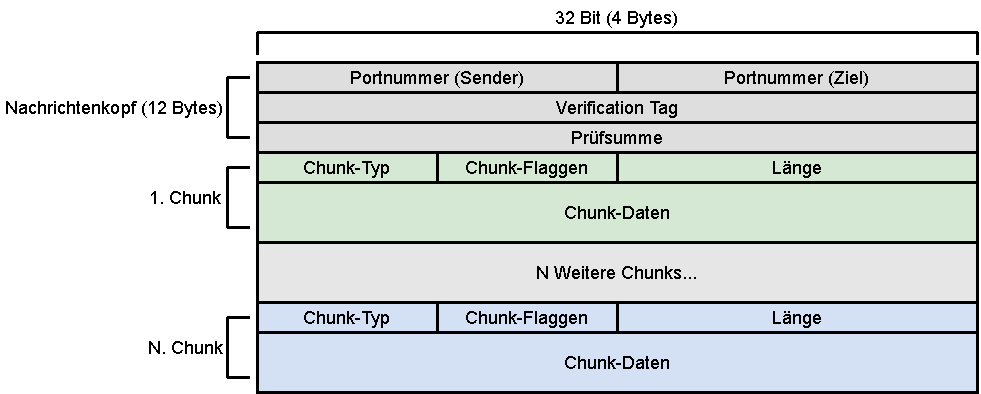
\includegraphics[width=0.95\textwidth]{bilder/PDF_SVG/SCTP_PACKET.pdf}
\caption{Aufbau eines \acs{SCTP}-Packets.}
\label{fig:sctpPacket}
\end{figure}

Ein \acs{SCTP}-Packet besteht aus einem Kopf- und einem Datenteil. Der Kopfteil beinhaltet neben dem Quell- und Zielport, sowie einer Prüfsumme noch ein \glqq{}Verification Tag\grqq{}, welches verwendet wird, um auf der Empfängerseite den Absender des Packets zu verifizieren, und eingehende Packete von denen früherer Verbindungen zu unterscheiden \cite{sctpRFC}.

Der Datenteil des Packets ist in sogenannte \glqq{}Chunks\grqq{}  aufgeteilt. Jedes \glqq{}Chunk\grqq{} besitzt dabei Informationen wie den Chunk-Typ, die Länge in Bytes, oder die Zugehörigkeit zu Datenströmen. Insgesamt existieren über 14 Chunk-Typen, von einfachen Daten-Chunks zu Chunks, welche Daten zur Kontrolle der Verbindung beinhalten \cite{sctpRFC}. Je nach verwendeten Erweiterungen des \acs{SCTP}-Protokolls kann die Anzahl der Chunk-Typen variieren. Alle Arten dieser \glqq Chunks\grqq{} zu beschreiben würde den Rahmen dieser Arbeit überschreiten. Die generelle Struktur eines Datenpackets ist Abbildung ~\ref{fig:sctpPacket} zu entnehmen. Die maximale größe eines \glqq{}Chunks\grqq{} ist dabei, aufgrund des zwei-Byte langen Längenfelds auf 65,535 Kilobyte limitiert.

\color{black}

\subsection{DTLS: Datagram Transport Layer Security}
Das \acf{DTLS}-Protokoll ist ein auf \acf{TLS} aufbauendes Protokoll zur Verschlüsselung von Daten in Datagram-basierenden Verbindungen. Im Gegensatz zu \acs{TLS}, welches für die Nutzung mit \acs{TCP} konzipiert wurde, kann \acs{DTLS} also auch über \acs{UDP} übertragen werden.\par

Da das von Datenkanälen genutzte \acs{SCTP}-Protokoll über keine eigene Verschlüsselung verfügt, und Verschlüsselung aller Daten eine zentrale Anforderung von \acs{WebRTC} darstellt, werden Daten über einen \acs{DTLS}-Tunnel zwischen den Verbindungspartnern ausgetauscht. Dieser Tunnel liegt auf dem \acf{UDP}. Die \acs{SCTP}-Verbindung eines Datenkanals läuft also nicht direkt auf dem \acf{IP}, sonder über einen \acs{DTLS}-Tunnel, welcher wiederrum auf \acs{UDP} liegt.

\section{Node.js}
Node.js ist eine kostenlose, plattformunabhängige JavaScript Laufzeitumgebung.
Diese ermöglicht das Ausführen von JavaScript Programmen außerhalb eines Browsers, zum Beispiel auf einem Server. Node.js ist Open-Source und kann kostenlos verwendet werden. Programme setzen sich aus sogenannten \textit{modules}, zu Deutsch Modulen, zusammen. Ein Modul kann dabei jegliche Funktionalität, wie zum Beispiel Klassen, Funktionen und Konstanten exportieren, welche dann wiederrum von weiteren Modulen oder Programmen verwendet werden können. Module können über das \textit{require}-Stichwort geladen werden. Node.js bietet integrierte Webserver-Funktionalität via dem \acs{HTTP}-Modul, welches das Erstellen eines Webservers ermöglicht \cite{nodejs}. Weiterhin bietet Node.js mit dem \glqq{}crypto\grqq{}-Modul kryptografische Funktionen, welche auf OpenSSL (Open Secure Socket Layer) basieren.\par 

Node.js ist in den Repositories aller aktuellen Linux-Distributionen enthalten\footnote{Weitere Informationen: \url{https://nodejs.org/en/download/package-manager/}}, und kann mit den entsprechenden Packetmanagern, beziehungsweise über die Website\footnote{Node.js Downloads: \url{https://nodejs.org/en/download/}} heruntergeladen und installiert werden.\par

\subsection{NPM: Node Package Manager}
Zur Verwaltung und zum Teilen von Packeten nutzt Node.js den \ac{NPM}. Ein Packet sind in diesem Kontext ein oder mehrere Module, gekoppelt mit allen Dateien, welche diese benötigen. Packete werden auf \textit{npmjs.com} gehostet. Die Liste der von einem Projekt verwendeten Module wird in der Datei \textit{package.json} gespeichert.

\subsection{Verwendete Node-Packete}
Neben den standartmäßig in Node.js enthaltenen \glqq{}http\grqq{}- und \glqq{}crypto\grqq{}-Modulen werden zwei weitere Packete genutzt: die \glqq{}socket.io\grqq{} Bibliothek und das \glqq{}express\grqq{}-Framework.

\subsubsection{socket.io}
\glqq{}socket.io\grqq{} ist eine Bibliothek, welche bidirektionale Echtzeitkommunikation zwischen einem Client und einem Server ermöglicht. Dazu nutzt Socket.io intern WebSockets\cite{socketio}. Ein WebSocket ermöglicht Kommunikation zwischen einem Client und einem Server. Der Datenaustausch findet dabei über das \ac{TCP} statt \cite{websocketRFC}. Das WebSocket \ac{API} wird von allen aktuellen Browsern unterstützt\footnote{vgl. \url{https://caniuse.com/mdn-api_websocket}, Stand: 08.04.2021}. Socket.io läuft auf einem Node.js Server\cite{socketio}.\par

Die Kommunikation zwischen Client und Server wird bei Socket.io über Events geregelt. Client und Server können Events -- definiert durch einen String -- mit angehängten Daten emittieren. Basierend auf dem Event-String wird dann auf der Empfängerseite eine Rückruffunktion aufgerufen, vorrausgesetzt diese ist definiert. Die Daten werden der Rückruffunktion als Parameter übergeben. Socket.io ermöglicht auf der Serverseite sowohl das Broadcasting an alle, beziehungsweise an ein Subset an Clients, als auch Unicasting an einen spezifischen Client \cite{socketio}.\par

Die Socket.io Bibliothek ist in eine Client-, und eine Serverseitige Bibliothek aufgeteilt. Die Clientseitige Bibliothek ermöglicht das Verbinden mit einem Node.js Server. Ein Client kann sowohl Events mit Daten emittieren, als auch Rückruffunktionen registrieren, mit welchen der Client Daten vom Server empfangen kann. Auf der Serverseite ist es möglich, bei Verbindungsaufbau Rückruffunktionen für einen neu verbundenen Client zu registrieren, welche bei dem Eingang von Daten je nach Event-Typ aufgerufen werden. Der Server kann ebenfalls Events an Clients emittieren.

\subsubsection{express}
\glqq{}express\grqq{} ist ein Node-Web-Framework, welches bei der Erstellung von Webanwendungen zum Einsatz kommt. Express agiert als Middleware zwischen einem \acs{HTTP}-Server und einer Webanwendung, und ermöglicht es, basierend auf \acs{HTTP}-Methoden und \acs{URL}s -- den sogenannten \glqq{}Pfaden\grqq{} -- verschiedene Aktionen auszuführen \cite{express}. Zudem bietet express weitere Funktionalitäten, wie das Bereitstellen von statischen Website-Daten, oder die Integration von \glqq{}Rendering-Engines\grqq{}, welche die Daten einer Website je nach Pfad dynamisch anpassen \cite{express}.

\chapter{WebRTC in Mehrspieler-Spielen}
\acs{WebRTC} wird bereits in einigen Browserbasierten Mehrspieler-Spielen, sowie Networking- und Spiel-Frameworks verwendet. In der Regel wird WebRTC dabei jedoch lediglich für Sprach- und Videokommunikation eingesetzt. Die Strategie- und Brettspiel Plattform \textit{Jocly} ist eine der ersten Plattformen, welche bereits seit 2013 \acs{WebRTC} nutzt, damit Spieler sich in Echtzeit über ihre Webcams beim Spielen sehen, sowie miteinander kommunizieren können (vgl. Abbildung~\ref{fig:jocly}) \cite{jocly2013}. Ähnlich verhält es sich bei einigen weiteren Frameworks, wie zum Beispiel \textit{Tabloro}\footnote{vgl. \url{https://github.com/fyyyyy/tabloro}}, einem Browserbasierten \glqq{}Tabletop\grqq{}-Spielsimulator. Diese Spiele und Frameworks nutzen eine Client-Server-Architektur für den regulären (nicht Video und Audio) Datenaustausch.\par

\begin{figure}[h]
\centering
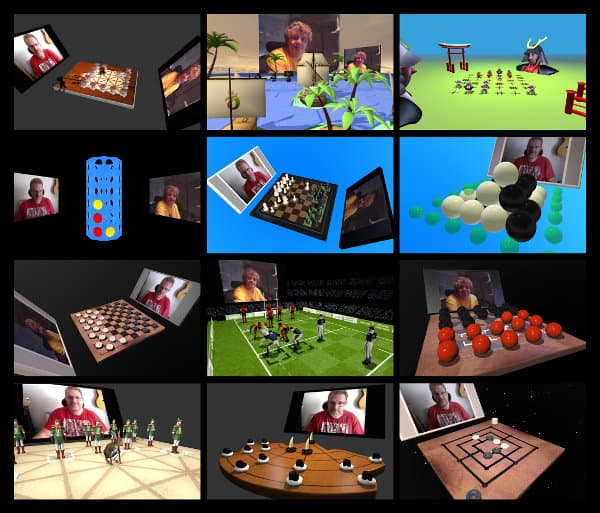
\includegraphics[width=0.70\textwidth]{bilder/jocly-games.jpg}
\caption{Einige Jocly-Spiele, mit WebRTC Videokommunikation.}
\source{\url{https://bloggeek.me/jocly-webrtc-interview/}}
\label{fig:jocly}
\end{figure}

Weiterhin existieren eine Reihe an prototypischen Spielen und Frameworks, welche \acs{WebRTC} zum Austausch von Daten nutzen. Bei diesen handelt es sich überwiegend um Echtzeitspiele wie das 2013 von Google entwickelte \textit{CubeSlam}. Abbildung~\ref{fig:cuubslam} zeigt dabei eine Bildschirmaufname eines CubeSlam-Spiels. CubeSlam nutzt \acs{WebRTC} Medienstreams, um Videodaten zu übertragen, und Datenkanäle, um die Spieldaten zwischen den Spielern zu synchronisieren. Auch der 2012 von Mozilla entwickelte First-Person-Shooter \textit{Bananabread}\footnote{vgl. \url{https://hacks.mozilla.org/2013/03/webrtc-data-channels-for-great-multiplayer/}} nutzt WebRTC zum Austausch von Spieldaten.\par

\begin{figure}[h]
\centering
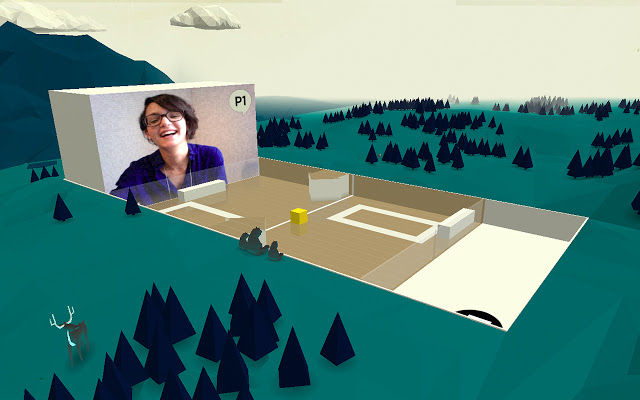
\includegraphics[width=0.70\textwidth]{bilder/cubeslam.jpg}
\caption{Google CubeSlam, mit integriertem WebRTC Videostream.}
\source{\url{https://experiments.withgoogle.com/cube-slam}}
\label{fig:cuubslam}
\end{figure}



Im Bereich der Rundenbasierten Brettspieleentwicklung im Browser findet WebRTC hingegen nur begrenzt Anwendung. Diese beschränkt sich primär auf die zuvor beschriebene Nutzung für Audio- und Videokommunikation.

\chapter{Konzept}
Dieses Kapitel befasst sich mit dem Verwendeten Konzept der Implementierung, Dabei wird primär auf die Anforderungen der Netzwerkstruktur eingegangen.

\section{Anforderungen}
Es soll ein System geschaffen werden, welches das Spielen des Brettspiels \glqq{}Mensch Ärgere Dich Nicht\grqq{} für mindestens vier Spieler ermöglicht. Die Anforderungen an das System gliedern sich in zwei Teile: Anforderungen an das Spiel an sich, und Anforderungen an die unterliegende Netzwerkstruktur.\par

\subsection{Anforderungen an die Netzwerkstruktur}
Die Spieler sollen sich an verschiedenen Geräten, sowie in verschiedenen Subnetzen befinden können. Der zum Spielablauf notwendige Datenaustausch soll über ein \acs{WebRTC}-Peer-To-Peer Netzwerk zwischen den Spielern stattfinden. Dies setzt die Verwendung von STUN- und TURN-Servern vorraus. Es muss mindestens ein STUN- und ein TURN-Server existieren. Der Datenaustausch zwischen Peers muss dabei zuverlässig und geordnet sein.\par

Dritte sollen die STUN- und TURN-Server nur zu deren vorgesehenem Zweck -- zum Spielen des Brettspiels -- in Verbindung mit der Webanwendung nutzen können. Dazu müssen für jeden Nutzer dynamische, spezifische, zeitlich begrenzte Anmeldedaten erstellt werden, mit welchen eine Verbindung zu den Servern möglich ist. Diese Daten müssen beim Betreten eines Spiels an den jeweiligen Spieler vergeben werden.\par

\label{section:weitere}
Damit mehr als ein Spiel zur gleichen Zeit stattfinden kann, müssen die Spieler in Teilmengen unterteilt werden. Zwischen den Spielern in einer solchen Teilmenge müssen Signalisierungsdaten zum Verbindungsaufbau austauschbar sein. Spieler müssen diesen Teilmengen beitreten, und die Teilmengen verlassen können. Eine Teilmenge repräsentiert dabei einen virtuellen \glqq{}Tisch\grqq{} oder \glqq{}Raum\grqq{}. Ein \glqq{}Raum\grqq{} muss zudem über einen Spieler verfügen, welcher Berechtigungen zum Entfernen von Spielern besitzt, falls ein unerwünschter Spieler beitritt oder betrügt.\par

\subsection{Anforderungen an die Clientseitigen WebRTC-Verbindungen}
Für jeden Peer muss ein Objekt existieren, welches sämtliche Verbindungen zu weiteren Peers verwaltet. Für jede Verbindung muss jeweils ein geordneter, zuverlässiger Datenkanal existieren. Es soll ein Event-Basiertes Nachrichtenprotokoll verwendet werden. Für verschiedene Events sollen -- ähnlich dem Syntax von socket.io -- Rückruffunktionen registrierbar sein können, die Parameter dieser Rückruffunktionen sollen dabei die Daten des Events beinhalten.

\subsection{Anforderungen an das Brettspiel}
Das Brettspiel soll durch das einfache Aufrufen einer Website spielbar sein. Die Webanwendung soll das Spielen einer virtuellen Nachbildung des Gesellschaftsspiels \glqq{}Mensch Ärgere Dich Nicht\grqq{} ermöglichen. Das Spiel muss von bis zu vier Spielern gleichzeitig spielbar sein. Spieler sollen dem Spiel beitreten und es während das Spiel noch läuft wieder verlassen können. Falls beim Verlassen eines Spielers noch Spieler vorhanden sind, so sollen diese weiterspielen können. 

\subsubsection{Betrug}
In Browserbasierten Webanwendungen ist es leicht, den JavaScript-Quellcode bei Laufzeit zu modifizieren. So können Spieler zum Beispiel unfaire Würfelergebnisse generieren, oder unerlaubte Spielzüge machen. Insbesondere die Würfelergebnisse lassen sich leicht manipulieren, ohne dass andere Spieler den Betrug überhaupt mitbekommen.\par

Spieler sollen daher nicht durch Modifikation von Script-Dateien betrügen können, ohne dass dies den anderen, nicht betrügenden Spielern angezeigt wird. Bei Benachrichtigung über den Betrug eines Spielers soll dieser Spieler vom, in Unterpunkt~\ref{section:weitere} beschriebenen, \glqq{}Host\grqq{}-Spieler aus dem Spiel entfernt werden können.\par

\subsubsection{Spielregeln}
Oh je das wird elend zu erklären, MÄDN ist leider etwas komplexer algorithmisch zu beschreiben als gedacht... evtl. nur Verweis auf die offiziellen Spielregeln?

\section{Server-Infrastruktur}
Für die Raum-Funktionalität, Signalisierungsmechanismen, sowie die Generierung von STUN- und TURN-Anmeldedaten müssen entsprechende Server existieren. Für die Implementierung werden alle diese Funktionen prototypisch in einem Server zusammengefasst.

\section{Peer-To-Peer Netzwerkarchitektur}
Bei der Netzwerkarchitektur des Peer-To-Peer Netzwerks kommen primär zwei Ansätze infrage: Das Authoritative-Peer-Modell, oder ein volles Peer-Netz.\par 

Das Authoritative-Peer-Modell folgt dem Authoritative-Server-Modell, mit dem Unterschied, dass die Funktionen des Servers dabei von einem der Peers übernommen werden. Es wird eine Stern-Netzwerktopographie erzeugt, wobei der sogenannte \glqq{}Host-Peer\grqq{} den zentralen Knoten bildet. Sämtlicher Datenaustausch läuft über den Host-Peer, welcher zudem die volle Authorität über den Spielstand besitzt. Die Client-Peers besitzen dabei nur den zur Darstellung des Spiels notwendigen, minimalen Spielstand. Der Vorteil dieses Modells ist die geringere Anzahl an Verbindungen im Netzwerk, sowie eine einfachere Entwicklung, da diese an das Authoritative-Server-Modell angelehnt werden kann. Problematisch ist jedoch der Single-Point-Of-Failure -- verliert der Host-Peer die Verbindung, so gehen alle Verbindungen sowie der Spielstand verloren. Für diese Fälle muss ein \glqq{}Host-Peer-Migrationsprozess\grqq{} existieren, um alle Verbindungen zu einem neu gewählten Host-Peer erneut zu erstellen. Existiert dieser nicht, so beendet das Verlassen des Host-Peers zwangsweise das Spiel.\par

Der Full-Mesh-Ansatz bildet das Gegenteil zum Authoritative-Peer-Modell. Hier verwaltet jeder Peer eine lokale Kopie des vollen Spielstands, und besitzt eine Verbindung zu jedem anderen Peer. Insbesondere bei Hohen Datenraten und einer hohen Anzahl an Peers skaliert diese Netzwerktopologie schlecht, was jedoch in diesem Fall aufgrund der geringen Spieleranzahl, sowie des geringen Datenvolumens praktisch irrelevant ist. Letztendlich wurde dieser Ansatz für die Implementierung der Netzwerkarchitektur gewählt, da dieser keine komplexen Host-Migrationsprozesse vorraussetzt.\par

\section{Zufallszahlen}
Ist die Netzwerktopographie eines Brettspiels ein Authoritative-Server-Modell, so ist es einfach, faire, unabhängige Zufallszahlen zu erstellen. Ein Client kann einfach eine Anfrage an den Server schicken, welcher eine Zahl generiert und an den Client zurückschickt. Macht der Spieler darauf einen Spielzug, so kann dieser vom Server mit Hinblick auf die zuvor generierte Zufallszahl validiert werden. In einem Full-Mesh Peer-Netzwerk ist dies nicht ohne weiteres möglich.\par

\subsection{Verteiltes Generieren von Zufallszahlen}
Ein naiver Ansatz zur Generation von Zufallszahlen ist daher, jeden Peer eine Zahl $z$ bis zu einem Wert $max$ generieren zu lassen, welche ausgetauscht und addiert werden. Anschließend ergibt $z \mod max$ eine Zahl, welche -- vorrausgesetzt mindestens einer der Peers hat eine zufällige Zahl generiert und nicht betrogen -- zufällig ist. Hier existiert jedoch das sogenannte \glqq{}Look-Ahead-Problem\grqq{}, wobei ein Peer einfach auf die Zufallszahlen aller anderen Peers warten kann, bevor dieser die eigene Zufallszahl abgeschickt hat. Basierend auf den Zufallszahlen der weiteren Peers kann der böswillige Peer nun eine Zahl abschicken, welche diesem ein gewünschtes Ergebnis -- verbunden mit einem Spielerischen Vorteil -- bringt. Für dieses Problem existieren Lösungsansätze wie das \glqq{}Lockstep-Protokoll\grqq{}, unter Nutzung von Commitment-Verfahren. Bei einem Commitment-Verfahren werden die zu sendenden Daten zuerst mit einem Passwort verschlüsselt und unter den Teilnehmern ausgetauscht. Sind alle verschlüsselten Daten ausgetauscht, so werden die Passwörter ausgetauscht. Es ist einem Peer somit nicht möglich, auf alle weiteren Zahlen zu warten, ohne vorher eine eigene Zahl erstellt zu haben.\par

\subsection{Seeded Random-Number-Generators}
Eine einfachere Methode zur Generierung von fairen Zufallszahlen in verteilten Systemen wie Peer-Netzwerken sind daher \glqq{}Seeded-Random-Number-Generators\grqq{}. Dabei lässt sich ein Zufallszahlengenerator mit einem Startwert, dem sogenannten \glqq{}Seed\grqq{} initialisieren. Der Generator erzeugt basierend auf diesem Seed eine Folge an Pseudozufallszahlen, welche bei der Nutzung des gleichen Seeds stets gleich ist. Um eine hinreichende Zufälligkeit der Zahlenfolge zu garantieren, ist der Seed in der Regel eine Zufallszahl, welche zum Beispiel einmalig von einem Server generiert werden kann. Besitzt jeder Peer den gleichen Seed, so muss nur die Aktion des Generierens an sich synchronisiert werden -- daraufhin generiert jeder Peer eine faire, unabhängige Pseudozufallszahl. Wichtig ist hierbei, dass der Spielstand zwischen den Peers unbedingt synchron gehalten werden muss. Generiert ein Teilnehmer eine Zahl zu viel oder zu wenig, so sind die Generatoren nicht mehr synchron. Dieser Ansatz bietet sich bei Brettspielen besonders an, da diese -- im Gegensatz zu Echtzeitspielen -- in der Regel in klar definierte \glqq{}Züge\grqq{} und \glqq{}Runden\grqq{} eingeteilt sind. Ein synchroner Spielstand zwischen den Spielern ist somit einfach beizubehalten.\par



\chapter{Design und Implementation}
Das Projekt gliedert sich primär in zwei Teile: Das Brettspiel \glqq{}Mensch Ärgere Dich Nicht\grqq{}, und die unterliegende \acs{WebRTC}- und Netzwerkinfrastruktur. Die Projektstruktur selbst ist in Abbildung~ \ref{table:projectfiles} beschrieben. Auf die Spiel- und Netzwerkspezifischen Script-Dateien wird in deren jeweiligen Sektionen weiter eingegangen.

\begin{table}[ht]
\centering
\begin{tabularx}{\textwidth}{lX}
\toprule
Dateipfad&Beschreibung\\
\midrule
/*&Grundverzeichnis des Servers\\
/Server.js&Diese Datei ist die ausführbare Script-Datei des Webservers. Hier wird der express-Webserver erstellt, sowie die WebSocket Verbindungen via socket.io, und die Spielräume verwaltet.\\
/utils.js&Hilfsfunktionen zum Generieren von TURN-Passdaten, Raum-IDs und Peer-IDs.\\
/config.json&Server-Konfiguration.\\
/package.json&NPM-Konfiguration.\\
\midrule
/public/*&Öffentliche Dateien, welche über den Webserver abgerufen werden können.\\
/public/index.html&HTML-Datei der Seite, auf welcher ein Spieler einen Raum erstellen oder beitreten kann.\\
/public/game.html&HTML-Datei der Spiel-Seite.\\
\midrule
/public/resources/*&CSS, Bild- und Scriptressourcen.\\
/public/resources/script/index.js&JS-Datei der Index-HTML-Seite.\\
/public/resources/script/game.js&JS-Datei der Spiel-HTML-Seite.\\
\midrule
/public/resources/script/network/*&Netzwerkspezifische Script-Dateien\\
/public/resources/script/game/*&Spielspezifische Script-Dateien\\
\bottomrule
\end{tabularx}
\caption{Struktur des Projektes.}
\label{table:projectfiles}
\end{table}

\section{Bereitstellungsplattform}
Zur Bereitstellung der in diesem Kapitel beschriebenen Server wird eine Virtuelle Maschine auf der Azure-Plattform genutzt. Azure ist eine Cloud-Computing-Plattform von Microsoft, welche sowohl Software-, Platform- und Infrastructure-As-A-Service (SaaS, PaaS, IaaS) anbietet.\par

Azure ermöglicht das Erstellen von Rechnenressourcen in der Cloud, in der Form von Virtuellen Maschinen. Dabei existieren verschiedene Ausführungen von Virtuellen Maschinen, welche sich beim dem eingesetzten Betriebssystem, sowie der \glqq{}Größe\grqq{} anpassen lassen. Die Größe gibt dabei den Arbeitsspeicher, die Anzahl der (virtuellen) Prozessorkerne, sowie die Art und Anzahl der Datenträger vor.\par

Für die prototypische Bereitstellung der Server wurde eine \acf{VM} der Größe \glqq{}B1s\grqq{} erstellt. Die B-Reihe ist dabei auf geringe Arbeitsbelastung ausgelegt. Eine B1s-VM verfügt über einen virtuellen Prozessorkern, ein Gigabyte Arbeitsspeicher und zwei Datenträger mit maximal 4 Gigabyte an temporärem Speicher. Für eine prototypische Bereitstellung, bei welcher nicht viel Serverlast zu erwarten ist, ist eine B1s-VM ausreichend.\par

Als Betriebssystem eignet sich praktisch jedes Betriebssystem, welches das bereitstellen von Servern ermöglicht. Azure bietet dabei viele verschiedene Linux-Distributionen und Windows-Server-Images. Als Betriebssystem wurde hier Ubuntu 18.04 LTS (Long-Term-Support, dt. Langzeitsupport) gewählt, primär da das Packet des genutzen STUN- und TURN-Servers in den Repositories von Ubuntu 18.04+ enthalten ist, und so einfach über den Packetmanager \textit{apt} installiert werden kann.\par

Der \acs{VM} muss zusätzlich eine öffentliche IP-Adresse zugewiesen werden, damit die auf der Maschine laufenden Server von Außen erreichbar sind. Für diese IP-Adresse lässt sich zudem ein Domain-Name in der Form
\lstset{style=STYLE_COMMAND_LINE_ARGUMENT_SINGLE_LINE}
\begin{lstlisting}[belowskip=-0.8 \baselineskip]
<DNS-Name>.<Region der VM>.cloudapp.azure.com
\end{lstlisting}
festlegen. Der für diese VM gewählte Domain-Name lautet somit:
\lstset{style=STYLE_COMMAND_LINE_ARGUMENT_SINGLE_LINE}
\begin{lstlisting}[belowskip=-0.8 \baselineskip]
ba-webrtc.westeurope.cloudapp.azure.com
\end{lstlisting}

\section{Implementation der Netzwerkinfrastruktur}
Die Netzwerkinfrastruktur ist in drei Teile geteilt: Der Webserver, welcher die Seiten bereitstellt und als Signalisierungskanal dient, die Clientseitige WebRTC-Implementation und die \acs{STUN}- und \acs{TURN}-Server. Zusammen bilden diese drei Komponenten das \glqq{}WebRTC-Dreieck\grqq{}.

\subsection{Implementation des Webservers}
Um das Verbinden von Peers via WebRTC zu ermöglichen, muss vorerst ein Signalisierungskanal existieren, welcher Nachrichten zwischen Peers weiterleiten kann. Die Art des Signal-Kanals ist dabei nicht vom WebRTC-Standard vorgegeben. Für die Implementierung wurde daher ein Signal-Server geschaffen, welcher WebSockets zur Datenübertragung nutzt. Der Server dient zusätzlich als Webserver, welcher das Brettspiel als Webanwendung bereitstellt, und die Nutzer in \glqq{}Räume\grqq{} unterteilt, damit mehr als ein Spiel zur gleichen Zeit stattfinden kann.\par

\subsubsection{Erstellen des Node-Servers}
Um einen Node-Server zu erstellen, muss der Node-Package-Manager über den Kommandozeilenbefehl

\lstset{style=STYLE_COMMAND_LINE_ARGUMENT_SINGLE_LINE}
\begin{lstlisting}[belowskip=-0.8 \baselineskip]
$ npm init
\end{lstlisting}

initialisiert werden. Dieser Befehl erstellt die \glqq{}package.json\grqq{}-Datei im momentanen Arbeitsordner. Zudem müssen die benötigten Packete via

\lstset{style=STYLE_COMMAND_LINE_ARGUMENT_SINGLE_LINE}
\begin{lstlisting}[belowskip=-0.8 \baselineskip]
$ npm install socket.io
$ npm install express
\end{lstlisting}

heruntergeladen werden. Daraufhin können diese Packete über die $require$-Funktion in ein Script eingebunden werden.

\subsubsection{express Web-Server}
Zur Erstellung des Webservers wird das \glqq{}express\grqq{}-Framework verwendet. Der Quellcode befindet sich in der \glqq{}Server.js\grqq{}-Datei, und ist in Abbildung~\ref{lst:express} abgebildet.

\vspace{11pt}
\lstset{language=js, style=STYLE_CODE_JS}
\begin{minipage}{\textwidth}
\begin{singlespace}
\begin{lstlisting}[caption={express Server -- Server.js}, captionpos=b, label={lst:express}]
const express = require('express');
const config = require('./config.json');

const app = express();
const server = require('http').Server(app);

app.use(express.static(config.server.public));

app.get('/', (req, res) => {
  res.status(200);
  res.sendFile(`${__dirname}${config.server.indexPage}`);
});

app.get('/game/*/', (req, res) => {
  res.status(200);
  res.sendFile(`${__dirname}${config.server.gamePage}`);
});

server.listen(config.server.listeningPort);
\end{lstlisting}
\end{singlespace}
\end{minipage}

Zuerst muss eine express-Anwendung über die $express()$-Funktion erstellt werden. Da für die Nutzung von socket.io allerdings ein \acs{HTTP}-Serverobjekt nötig ist, wird dieses in Zeile 5 erstellt. Dabei wird die express-Anwendung als Parameter bei der Servererstellung mitgegeben. Die express-Anwendung nutzt nun diesen \acs{HTTP}-Server für die Webserver-Funktionalität.\par

Da die \acs{HTML}-Dateien die notwendingen Scripts aus anderen Dateien importieren, müssen diese via \acs{URL} vom Webserver abrufbar sein. Die Funktion $app.use$ erlaubt es, Dateien via \acs{URL} öffentlich bereitzustellen. In Zeile 7 wird daher der Inhalt des \glqq{}public\grqq{}-Ordners statisch zur Verfügung gestellt.\par

Des Weiteren werden in Zeile 9 und 14 die Pfade definiert, auf welchen die \acs{HTML}-Dateien abrufbar sind. Ruft ein Nutzer die Basis-\acs{URL} des Servers auf, so sendet der Server die \textit{index.html}-Datei. Ruft ein Nutzer den Pfad \textit{<Basis-Server-URL>/game/<Raum-ID>/} auf, so wird dieser auf die Raum-Seite (\textit{room.html}) verwiesen. Dies bewirkt, dass ein Nutzer direkt über eine \acs{URL} einem Spiel beitreten kann, und nicht über die Index-Seite beitreten muss. Die Dateipfade sind in der Server-Konfigurationsdatei definiert.

Zuletzt muss in Zeile 19 noch der Port definiert werden, über welchen der Server von außen ansprechbar sein soll. Dieser ist ebenfalls via der Konfigurationsdatei definierbar. Wichtig ist, dass dieser Port des Servers, auf welchem der Webserver läuft, weitergeleitet ist [siehe: Aufsetzen der Server (oder so, // todo!!!)].

\subsubsection{socket.io}
Auf der Serverseite muss eine socket.io-Instanz erstellt werden. Diese nutzt den gleichen \acs{HTTP}-Server wie die express-Anwendung. Baut ein Client über die Clientseitige socket.io-Bibliothek eine Verbindung auf, so wird auf der Serverseite das \textit{connection}-Event ausgelöst, welches den Socket des Clients als Parameter enthält. Innerhalb der Rückruffunktion dieses Events müssen alle Rückruffunktionen für diesen Socket registriert werden. Der dazu notwendige Quellcode ist in Abbildung~\ref{lst:socketioserver} abgebildet.

\vspace{5pt}
\lstset{language=js, style=STYLE_CODE_JS}
\begin{minipage}{\textwidth}
\begin{singlespace}
\begin{lstlisting}[caption={Initialisierung des socket.io Servers -- Server.js}, captionpos=b, label={lst:socketioserver}]
[...]
const server = require('http').Server(app);
const io = require('socket.io')(server);
[...]
io.sockets.on('connection', (socket) => {
  [...] // Rueckruffunktionen
}
\end{lstlisting}
\end{singlespace}
\end{minipage}

Auf der Client-Seite muss zuerst die Clientseitige socket.io-Bibliothek eingebunden werden. Läuft socket.io auf dem gleichen Server wie der express-Webserver, so stellt socket.io die Clientseitige Script-Datei auf dem Pfad \textit{/socket.io/socket.io.js} statisch bereit. Die Datei wird im Header der jeweiligen \acs{HTML}-Datei über ein \textit{script}-Tag eingefügt:
\lstset{style=STYLE_COMMAND_LINE_ARGUMENT_SINGLE_LINE}
\begin{lstlisting}[belowskip=-0.8 \baselineskip]
<script src="/socket.io/socket.io.js"></script>
\end{lstlisting}
\par

\vspace{11pt}
Clientseitig stellt socket.io die \textit{io}-Funktion zur Verfügung, welche die Adresse des zugehörigen socket.io-Servers als Parameter nimmt. Die Funktion gibt die Socket-Instanz des Clients zurück. Das \textit{connect}-Event wird bei erfolgreicher Verbindung zum Server ausgelöst. Der hierzu notwendige Quellcode ist in Abbildung~\ref{lst:socketioclient} abgebildet.

\vspace{5pt}
\lstset{language=js, style=STYLE_CODE_JS}
\begin{minipage}{\textwidth}
\begin{singlespace}
\begin{lstlisting}[caption={Clientseitiger Verbindungsaufbau -- game.js}, captionpos=b, label={lst:socketioclient}]
$(document).on('DOMContentLoaded', () => {
  const socket = io('http://ba-webrtc.westeurope.cloudapp.azure.com:1234');
  const roomID = window.location.pathname.split('/')[2];
  socket.on('connect', () => {
    socket.emit('game-room-join', roomID);
  );
  [...] // Rueckruffunktionen
)
\end{lstlisting}
\end{singlespace}
\end{minipage}

Das \textit{connect}-Event wird nicht nur beim ersten Verbindungsaufbau, sondern auch bei jeder Neuverbindung aufgerufen. Um zu vermeiden, dass Rückruffunktionen mehrfach registriert werden, werden diese außerhalb der \textit{connect}-Rückruffunktion erstellt. 

\subsection{Implementation der Peer-To-Peer Funktionalität}
Zur Verwaltung der Peer-To-Peer-Funktionalität werden \glqq{}Peer\grqq{}-Objekte verwendet. Jeder Client besitzt dabei ein Peer-Objekt. Der Peer verwaltet die RTCPeerConnections, sowie die zugehörigen Datenkanäle. Es ist dem Peer möglich, ähnlich dem socket.io-Syntax Rückruffunktionen zu erstellen, welche bei Erhalt von Daten je nach Event aufgerufen werden.\par

\subsubsection{Eventbasiertes Nachrichtenprotokoll}
Der von den Peer-Objekten zum Datenaustasuch verwendete Syntax ist an den Syntax von socket.io angelehnt. An einem Peer lassen sich über die \textit{on}-Funktion Rückruffunktionen registrieren (vgl. Abbildung~\ref{lst:registerCallback}). Diese registriert die Funktion in einem Map-Objekt.\par

\vspace{5pt}
\lstset{language=js, style=STYLE_CODE_JS}
\begin{singlespace}
\begin{lstlisting}[caption={Funktion zur Registrierung von Rückruffunktionen -- Peer.js}, captionpos=b, label={lst:registerCallback}]
Peer.prototype.on = function(e, callback) {
  this.callbacks[e] = callback;
}
\end{lstlisting}
\end{singlespace}

Die \textit{broadcast}-Funktion emittiert ein Event an alle Peers, zu welchen der Datenkanal offen ist (vgl. Abbildung~\ref{lst:broadcastEvent}). Zudem existiert die \textit{emit}-Funktion, welche ein Event nur an einen Peer emittiert. Das Format des Nachrichtenprotokolls ist Zeile 3 zu entnehmen: Jede Nachricht besitzt jeweils einen Event-String und ein Array an Daten.\par

\vspace{5pt}
\lstset{language=js, style=STYLE_CODE_JS}
\begin{singlespace}
\begin{lstlisting}[caption={Funktion zum Emittieren eines Events -- Peer.js}, captionpos=b, label={lst:broadcastEvent}]
Peer.prototype.broadcast = function(e, ...args) {
  Object.values(this.connections).forEach((connection) => {
    connection.dc.send(JSON.stringify({event: e, data: args}));
  });
}
\end{lstlisting}
\end{singlespace}

Bei Empfang einer Nachricht wird die Rückruffunktion, welche für das Event registriert ist, ausgeführt (vgl. Abbildung~\ref{lst:receiveMessage}). Zudem wird die Peer-ID des Peers, welcher das Event emittierte als weiterer Funktionsparameter angehängt.\par

\vspace{5pt}
\lstset{language=js, style=STYLE_CODE_JS}
\begin{singlespace}
\begin{lstlisting}[caption={Funktion bei Erhalt einer Nachricht -- Peer.js}, captionpos=b, label={lst:receiveMessage}]
Peer.prototype._receiveMessage = function(e, remotePeerId) {
  const message = JSON.parse(e.data);
  if (message.event && this.callbacks[message.event]) {
    this.callbacks[message.event](...message.data, remotePeerId);
  }
}
\end{lstlisting}
\end{singlespace}

\subsubsection{Signalisierungsprotokoll}
Zur Signalisierung wird ein simples, proprietäres Protokoll verwendet. Eine Signal-Nachricht besitzt immer eine Quell-Peer-ID, eine Ziel-Peer-ID, eine Nachrichtenart, und die eigentlichen \acs{SDP}-Daten des Signals. Dabei wird zwischen den Signal-Typen \textit{offer}, \textit{answer} und \textit{ice-candidate} unterschieden. Die Signalnachrichten werden als \acs{JSON} encodiert und über den Signalisierungskanal weitergeleitet (siehe:~\ref{section:signalisierungskanal} Signalisierungskanal).\par

\vspace{5pt}
\lstset{language=js, style=STYLE_CODE_JS}
\begin{singlespace}
\begin{lstlisting}[caption={Format des Signalisierungsprotokolls}, captionpos=b, label={lst:protocoll}]
{
    source : <Peer-ID>,
    target : <Peer-ID>,
    type : 'offer' | 'answer' | 'ice-candidate',
    data : <SDP-Daten>
}
\end{lstlisting}
\end{singlespace}

Für ausgehende Signalnachrichten wird die \textit{signal}-Funktion des Peers verwendet. Diese muss bei Erstellen des Peer-Objekts registriert werden und Daten an das Signalisierungsmedium schicken. Werden Daten über den Signalisierungskanal erhalten, so muss die \textit{onsignal}-Funktion aufgerufen werden (vgl. Abbildung~\ref{lst:clientroomjoin}).

\subsubsection{Verbindungen und Datenkanäle}
Zum Verbindungsaufbau wird die \textit{connect}-Funktion (Abbildung~\ref{lst:connectfunction}) verwendet. Als Argument nimmt diese die Peer-ID des Peers, zu welchem eine Verbindung aufgebaut werden soll. Die RTCPeerConnection wird in der Hilfsmethode \textit{createConnection} des Peers erstellt, da diese Funktionalität auch auf der Empfängerseite bei Erhalt einer \acs{JSEP}-Anfrage verwendet wird.\par

\vspace{5pt}
\lstset{language=js, style=STYLE_CODE_JS}
\begin{minipage}{\textwidth}
\begin{singlespace}
\begin{lstlisting}[caption={\textit{connect}-Funktion -- peer.js}, captionpos=b, label={lst:connectfunction}]
Peer.prototype.connect = function(remotePeerId) {
  const connection = this._createConnection(remotePeerId);
  this.connections[remotePeerId] = connection;

  connection.createOffer().then((offer) => {
    this.signal(this._createSignal('offer', offer, remotePeerId));
    connection.setLocalDescription(offer);
  }).catch((e) => console.error(e));
}
\end{lstlisting}
\end{singlespace}
\end{minipage}

Nach dem Erstellen der RTCPeerConnection wird der \acs{JSEP}-Anfrage-Antwort Prozess zwischen den Peers eingeleitet. In Zeile 5 wird die Anfrage erstellt, in Zeile 6 wird diese dem Signalisierungsprotokoll entsprechend verpackt und über den Signalisierungskanal weitergeleitet. Zuletzt muss in Zeile 7 die lokale Konfiguration des Peers -- die SDP-Daten der Anfrage -- gesetzt werden.

\vspace{5pt}
\lstset{language=js, style=STYLE_CODE_JS}
\begin{minipage}{\textwidth}
\begin{singlespace}
\begin{lstlisting}[caption={Erstellen von Verbindungen und Datenkanälen -- peer.js}, captionpos=b, label={lst:makertcpeerconnection}]
Peer.prototype._createConnection = function(remotePeerId) {
  const connection = new RTCPeerConnection(this.rtcConfiguration);

  const channel = connection.createDataChannel('game', {
    negotiated : true,
    id : i,
    ordered : true,
    maxRetransmits : null
  });
  channel.onmessage = (e) => this._receiveMessage(e);
  // [...]
  connection.onicecandidate = (e) => {
    this.signal(this._createSignal('ice-candidate', e.candidate, remotePeerId));
  }
 
  connection.dc = channel;
  return connection;
}
\end{lstlisting}
\end{singlespace}
\end{minipage}

Der Quellcode zur Erstellung der RTCPeerConnection und des Datenkanals ist Abbildung~\ref{lst:makertcpeerconnection} zu entnehmen. Die Konfiguration der RTCPeerConnection beinhaltet die vom Webserver bei Raumbeitritt erhaltenen STUN- und TURN-Serveradressen, sowie deren Nutzerdaten zur Authentifizierung. In den Zeilen 4 bis 10 wird ein Datenkanal mit dem Namen \textit{game} erstellt. Die einzelnen Einstellungen werden in Tabelle~\ref{table:dataChannelConfig} beschrieben.

\begin{table}[ht]
\centering
\begin{tabularx}{\textwidth}{llX}
\toprule
Konfiguration&Wert&Beschreibung\\

\midrule
negotiated&true&Da die Anwendung symmetrisch ist -- beide Peers wissen, dass exakt ein geordneter, zuverlässiger Datenkanal erstellt werden soll -- wird ein im vorab vereinbarter Datenkanal verwendet. Hier ist wichtig, dass die Konfiguration des Kanals auf beiden Seiten exakt übereinstimmt.\\
id&0&Die numerische ID des Datenkanals, bei im Vorab vereinbarten Datenkanälen muss diese gegeben sein und zwischen beiden Peers übereinstimmen.\\
ordered&true&Das unterliegende \acs{SCTP}-Protokoll soll die Nachrichten geordnet absenden und erhalten.\\
maxRetransmits&null&Ist dieser Wert nicht gesetzt, so versucht das  \acs{SCTP}-Protokoll so lange ein Packet abzuschicken, bis dieses beim Empfänger angekommen ist.\\
\bottomrule

\end{tabularx}
\caption{Konfiguration der Datenkanäle.}
\label{table:dataChannelConfig}
\end{table}

Bei Erhalt eines \acs{ICE}-Kandidaten in der \textit{onicecandidate}-Rückruffunktion wird dieser über den Signalisierungskanal an den externen Peer gesendet.\par

Bei Erhalt einer Signalnachricht wird diese in der \textit{onsignal}-Funktion verarbeitet. Der Quellcode ist in Abbildung~\ref{lst:onsignal} abgebildet. Bei Erhalt einer Anfrage wird die RTCPeerConnection erstellt und die externe Konfiguration gesetzt. Daraufhin wird die Antwort erstellt und über die \textit{signal}-Funktion an den externen Peer weitergeleitet. Zuletzt wird die Antwort als lokale Konfiguration der Verbindung gesetzt. Bei Erhalt einer Antwort wird diese als die externe Konfiguration der RTCPeerConnection gesetzt. Bei Erhalt eines \acs{ICE}-Kandidaten wird dieser über die \textit{addICECandidate}-Funktion der RTCPeerConnection hinzugefügt.

\vspace{5pt}
\lstset{language=js, style=STYLE_CODE_JS}
\begin{singlespace}
\begin{lstlisting}[caption={Funktion zum Verarbeiten von Signalnachrichten -- Peer.js}, captionpos=b, label={lst:onsignal}]
Peer.prototype.onsignal = function(e) {
  switch(e.type) {
    case 'offer':
      const connection = this._createConnection(e.src);
      this.connections[e.src] = connection;
      connection.setRemoteDescription(e.data).then(() => {
        return connection.createAnswer();
      }).then((answer) => {
        this.signal(this._createSignal('answer', answer, e.src));
        connection.setLocalDescription(answer);
      });
      break;
    case 'answer':
      this.connections[e.src].setRemoteDescription(e.data);
      break;
    case 'ice-candidate':
      this.connections[e.src].addIceCandidate(e.data);
      break;
  }
}
\end{lstlisting}
\end{singlespace}

\subsection{Raum-Verwaltung}
Das Spiel \glqq{}Mensch Ärgere Dich Nicht\grqq{} kann maximal von vier Spielern gespielt werden. Damit mehr als ein Spiel gleichzeitig gespielt werden kann, müssen Spieler in \glqq{}Räume\grqq{} unterteilt werden. Ein Raum besitzt dabei eine Liste an bis zu vier Sets an Spielerdaten, eine Raum-ID und eine Host-ID. Bei der Host-ID handelt es sich um die Socket-ID des Spielers, welcher den Raum zuerst betritt. Dieser hat als einziger Spieler die Befugnis, weitere Spieler aus dem Raum zu entfernen. Spielerdaten enthalten jeweils die Peer-ID eines Spielers, einen Namen und die Spielfarbe des Spielers.

\subsubsection{Erstellen eines Raums}
\vspace{5pt}
\lstset{language=js, style=STYLE_CODE_JS}
\begin{singlespace}
\begin{lstlisting}[caption={Event zum Erstellen eines Raums -- Server.js}, captionpos=b, label={lst:imamakedaroom}]
const utils = require('./utils.js');
[...]
const rooms = {}
const playerSockets = {}

io.sockets.on('connection', (socket) => {
  socket.on('game-room-create', () => {
    const id = utils.generateRoomID(rooms);
    rooms[id] = {
      id : id, // easier to identify room by player
      players : [],
      started : false,
      host : null
    };
    [...]	
    socket.emit('game-room-created', id);
  });
  [...]
}
\end{lstlisting}
\end{singlespace}

Erstellt ein Nutzer einen Raum, so sendet dieser das \textit{game-room-create}-Event zum Server (vgl. Abbildung~\ref{lst:imamakedaroom}). Der Server generiert eine vierstellige Zeichenkette, welche als Raum-ID dient. Mit dieser wird in Zeile 10 ein Raum-Objekt erzeugt, welches die zuvor beschriebenen Daten enthält. Zudem speichert das Raum-Objekt, ob das Spiel in diesem Raum bereits gestartet ist. Ist der Raum erstellt, so wird ein Event an den erstellenden Client zurückgeschickt, um diesem mitzuteilen, dass der Raum nun beitretbar ist.\par

\subsubsection{Beitritt eines Raums}

Das Betreten eines Raums ist über das \textit{game-room-join}-Event geregelt. Versucht ein Nutzer einem Raum beizutreten, so sendet dieser das Event an den Server (vgl. Abbildung~\ref{lst:join}). Falls der Raum noch keinen Host-Spieler besitzt, so wird der erste Beitretende Spieler in Zeile 17 zum Host ernannt. Bei erfolgreichem Beitritt erhält der Nutzer, wie in Zeile 20 zu sehen, das \textit{game-room-joined}-Event zurück, welches sämtliche, zum Verbindungsaufbau mit den anderen Spielern des Raums, benötigten Daten enthält. Dazu gehören das Array der weiteren Spieler im Raum, die eigene Peer-ID und die Zugangsdaten zu den \acs{STUN}- und \acs{TURN}-Servern. Zusätzlich wird dem Nutzer mitgeteilt, ob dieser der Host des Raums ist. Zudem werden in Zeile 27--29 alle weiteren Spieler des Raums benachrichtigt, dass ein weiterer Spieler beigetreten ist.\par

In den Spielregeln von \glqq{}Mensch Ärgere Dich Nicht\grqq{} ist geregelt, dass beim Spielen mit zwei Spielern die Farben Gelb und Rot gewählt werden sollen, damit die Spieler gegenüberstehende Startfelder haben. Daher werden die Spieler beim Betreten eines Raums nicht nach aufsteigender Reihenfolge in das Spieler-Array eingefügt, sondern nach der in Zeile 1 definierten Reihenfolge [0, 2, 1, 3]. Ab Zeile 8 wird dieses Array durchlaufen. Ist ein Array-Index nicht definiert, so wird der neu beigetretene Spieler an diese Stelle des Spieler-Arrays gesetzt.\par

\begin{table}[ht]
\centering
\begin{tabular}[t]{lc}
\toprule
Spieler-Index&Farbe im Spiel\\
\midrule
0&Gelb\\
1&Grün\\
2&Rot\\
3&Schwarz\\
\bottomrule
\end{tabular}
\caption{Spielerfarben.}
\label{table:playercolors}
\end{table}

Dazu wird in Zeile 10 zuerst eine Peer-ID generiert, welche zu Signalisierungszwecken genutzt wird. Die \glqq{}Farbe\grqq{} des Spielers ist dabei der Index des Spielers im Spieler-Array (vgl. Tabelle~\ref{table:playercolors}).\par

\vspace{11pt}
\lstset{language=js, style=STYLE_CODE_JS}
\begin{singlespace}
\begin{lstlisting}[caption={Event zum Betreten eines Raums -- Server.js}, captionpos=b, label={lst:join}]
const PLAYER_SLOT_PRIORITY = [0, 2, 1, 3];
[...]
io.sockets.on('connection', (socket) => {
  [...]
  socket.on('game-room-join', (roomID) => {
    const room = rooms[roomID];
    [...]
    for (let i = 0; i < 4; i++) {
      if (!room.players[PLAYER_SLOT_PRIORITY[i]]) {
        const peerID = utils.uuid4();
        const color = PLAYER_SLOT_PRIORITY[i];

        playerSockets[peerID] = socket.id;
        room.players[color] = {peerID : peerID, color : color};

        if (!room.host) {
          room.host = socket.id;
        }

        socket.emit('game-room-joined', 
          room.players, 
          peerID, 
          utils.generateTURNCredentials(socket.id), 
          room.host === socket.id
        );

        room.players.forEach((player) => {
          socket.to(playerSockets[player.peerID]).emit('game-room-client-joining', peerID, color)
        });
        break;
      }
    }
  });
  [...]
}
\end{lstlisting}
\end{singlespace}

Der Zugehörige Clientseitige Quellcode ist Abbildung~\ref{lst:clientroomjoin} zu entnehmen. Bei Beitritt eines Raums wird zuerst das Peer-Objekt erstellt, welches die \acs{WebRTC} Verbindungen und Datenkanäle verwaltet (siehe [TODO: REF]). Zudem wird in Zeile 3 die Funktion für ausgehende Signale gesetzt. Diese nutzt die socket.io-Verbindung zur Datenübertragung. In Zeile 4 wird die Rückruffunktion für das \textit{signal}-Event erstellt, welche die Signaldaten an \textit{onsignal}-Funktion des Peer-Objekts weitergibt. In Zeile 6 bis 9 wird das Spiel an sich erstellt und initialisiert. Tritt ein weiterer Spieler dem Spiel bei, so wird die in Zeile 11 definierte Rückruffunktion ausgeführt. Wichtig beim Beitritt eines neuen Spielers ist, dass die Zufallsfunktion des Spiels für alle Spieler mit einem neuen Seed initialisiert wird. Ansonsten ist der Zufallszahlen-Generator des neu beigetretenen Spielers nicht synchron mit denen der weiteren Spieler.

\vspace{11pt}
\lstset{language=js, style=STYLE_CODE_JS}
\begin{singlespace}
\begin{lstlisting}[caption={Raumbeitritt auf der Client-Seite -- game.js}, captionpos=b, label={lst:clientroomjoin}]
socket.on('game-room-joined', (players, started, seed, peerID, servers, isHost) => {
  const peer = new Peer(peerID, servers, /* [...] */);
  peer.setSignalFunction((data) => socket.emit('signal', roomID, data.target, data)); 
  socket.on('signal', (e) => peer.onsignal(e));

  const game = new Game(/* [...] */);
  socket.on('game-start', (seed) => game.start(seed));
  started ? game.start(seed) : game.seed(seed);
  game.render();

  socket.on('game-room-client-joining', (seed, peerID, color) => {
	// [...]
    game.seed(seed);
    game.addPlayer(new Player(color, false));
  });
  // [...]
  players.forEach((player) => {
    player.peerID === peerID 
      ? game.localPlayerColor = player.color 
      : peer.connect(player.peerID);
      
    game.addPlayer(new Player(player.color, game.localPlayerColor === player.color));
  });
});
\end{lstlisting}
\end{singlespace}

Um Signalisierungsbedingte \glqq{}Race-Conditions\grqq{} beim Verbindungsaufbau zwischen Peers zu vermeiden, ist der zuletzt dem Raum beigetretene Peer stets der Peer, welcher die Verbindung zu anderen Peers initiiert. In Zeile 20 wird -- vorrausgesetzt die Peer-ID des Spielers ist nicht gleich der Peer-ID des lokalen Peers -- eine Verbindung über die \textit{connect}-Funktion zu jedem anderen Spieler im Raum erzeugt. Zuletzt müssen die Spieler dem Spieler-Array des Spiel-Objektes hinzugefügt werden.

\subsubsection{Weitere Raumspezifische Events}
\begin{table}[ht]
\centering
\begin{tabularx}{\textwidth}{lX}
\toprule
Event&Beschreibung\\

\midrule
game-room-join-failed&Wird vom Server zurückgegeben, wenn der Raum, dem der Client beitreten will, nicht verfügbar oder voll ist.\\
game-room-client-leaving&Wird vom Server an alle Spieler eines Raums gesendet, wenn ein Spieler den Raum verlässt.\\
game-room-host-migration&Ausgelöst vom Server, wenn der Host eines Raums diesen verlässt. Die Socket-ID des neuen als Host agierenden Spielers wird als Parameter dieses Events mitgegeben.\\
\bottomrule

\end{tabularx}
\caption{Weitere Raumspezifische Events.}
\label{table:otherevents}
\end{table}

Des weiteren existieren Events, welche das Verlassen von Räumen, entweder durch den Nutzer manuell ausgelöst, oder bedingt durch Verbindungsverlust, behandeln. Verlässt ein Spieler einen Raum, so erhalten alle verbliebenen Spieler ein Event darüber. Verlässt der Host-Spieler den Raum, so geht der Host-Status auf den nächsten Spieler im Spieler-Array über. Verlässt der letzte verbleibende Spieler den Raum, so wird dieser entfernt. Diese Events sind in Tabelle~\ref{table:otherevents} zusammengefasst.\par

\subsection{Signalisierungskanal}
\label{section:signalisierungskanal}
Das Weiterleiten von Signalisierungsnachrichten zwischen Peers wird über die gleiche socket.io-Verbindung geregelt, wie die Raumverwaltung. Dazu wird das \textit{signal}-Event verwendet. Zur Signalisierung muss dabei immer die ID des Raums angegeben werden, in welchem die Signal-Nachricht weitergeleitet werden soll. Zudem muss die Peer-ID des Ziel-Peers angegeben werden. Existieren Raum und Peer, so wird das \textit{signal}-Event an diesen weitergeleitet. Abbildung~\ref{lst:signalserver} zeigt die Serverseitige Rückruffunktion des \textit{signal}-Events.

\vspace{11pt}
\lstset{language=js, style=STYLE_CODE_JS}
\begin{singlespace}
\begin{lstlisting}[caption={Event zum Weiterleiten eines Signals -- Server.js}, captionpos=b, label={lst:signalserver}]
io.sockets.on('connection', (socket) => {
  [...]
  socket.on('signal', (roomID, targetID, e) => {
    const room = rooms[roomID];

    if (room) {
      const target = room.players.find((player) => && player.peerID === targetID);
      if (target) {
        socket.to(playerSockets[target.peerID]).emit('signal', e);
      }
    }
  });
  [...]
}
\end{lstlisting}
\end{singlespace}

\section{Aufsetzen und Konfiguration eines STUN und TURN Servers}


\chapter{Evaluation}
%\input{}
\chapter{Zusammenfassung und Ausblick}
%\input{}

%%%Ab hier werden die einzelnen Kapitel als extra .tex Dateien angehängt
%%%Die Kapitel brauchen dabei keine Formatierungen, nur Überschriften etc.
%%%Alle .tex in einem Ordner%%%
%\input{}

\begin{singlespace}
\bibliography{30_Literaturverzeichnis.bib}
\end{singlespace}
\clearpage

%\chapter{Anhang}
\end{document}